\chapter{Topologia generale}

La motivazione di topologia deriva da un ulteriore ammorbimento degli assiomi degli spazi metrici. In particolare se si considerano le palle di uno spazio metrico gli intorni aperti della topologia talvolta la topologia si dice metrizzabile (a seguire definizione). Analogamente data una distanza si può indurre una topologia. In particolare non tutte le topologie sono metrizzabili. 

\begin{definition}
	Sia $X \neq \varnothing$. Una struttura topologica su $X$ o semplicemente topologia su $X$ (o di $X$) è una famiglia $\tau$ di sottoinsiemi di $X$, cioé $\tau \subset 2^X$, che soddisfa le seguenti proprientà
	\begin{enumerate}
		\item $\varnothing, X \in \tau$
		\item $\tau$ è stabile per unione arbitraria. Ovvero 
		\begin{equation*}
			\bigcup_{i \in I} A_i \in \tau 	
		\end{equation*}
		dove $I$ è un qualsiasi insieme indicizzante e $\forall i. \; A_i \in \tau$.
		\item $\tau$ è stabile per intersezioni finite. Ovvero 
		\begin{equation*}
			\bigcap^n_{i=1} A_i \in \tau
		\end{equation*}
		dove $\forall i. \; A_i \in \tau$.
	\end{enumerate} 
\end{definition}

\begin{remark}
	È ovvio che l'ultima condizione si può riscrivere come segue: dati $A_1, A_2 \in \tau$ allora $A_1 \cap A_2 \in \tau$. Infatti per induzione si riottiene il terzo assioma. 
\end{remark}

\begin{definition}
	Sia $\tau$ una topologia su $X$ allora la coppia $(X, \tau)$ su chiama \textbf{spazio topologico}. $X$ si chiama \textbf{supporto dello spazio topologico}. Sia $A \in \tau$ allora $A$ si chiama \textbf{sottoinsieme aperto di $(X,\tau)$} o aperto di $\tau$ oppure aperto di $X$ (se $\tau$ è implicitamente definita). 	
\end{definition}

Poiché negli esempi a seguire dimostreremo che alcune semplici topologie possono essere metrizzabili, devo definire cosa intendo dire.
\begin{definition}
	Uno spazio topologico $(X,\tau)$ si dice metrizzabile se esiste una distanza $\morphism{d}{X\times X}{\R}$ tale che gli insiemi aperti indotti da $d$ sono gli stessi elementi di $\tau$. In particolare la topologia indotta da $d$, $\tau_d  = \tau$. 
\end{definition}

\begin{example}
\begin{enumerate}
	\item Sia $(X,d)$ uno spazio metrico e sia la famiglia $\tau_d$ degli aperti di $X$ rispetto a $d$. Allora $(X,\tau_d)$ formano uno spazio topologico. 
	\item[Topologia banale] La topologia più povera in assoluto è la topologia banale, ovvero $\tau = \left\{\varnothing, X\right\}$. Inoltre la topologia banale non è metrizzabile se non nel caso in cui $X = \left\{x\right\}$ ovvero sia un singoletto. Infatti sia $d$ una distanza su $X$ e sia $X = \left\{p,q\right\}$ allora per ogni $\rho > 0 \; . \; q \in B_\rho(p)$ per cui $d(p,q) = 0$ ma poiché $d$ è una distanza ottengo che $p=q$, contraddicendo il fatto che $p \neq q$. 
	\item[Topologia discreta] Dall'altra parte della barricata c'è la topologia discreta ovvero $\tau = 2^X$ che è la più ricca topologia possibile (infatti se $\tau$ è una topologia ho che $\tau \subseteq 2^X$). È ovviamente una topologia e vale anche l'assioma della stabilità per intersezioni di famiglie arbitrarie. Inoltre è sempre metrizzabile per ogni $X \neq \varnothing$. Infatti basta prendere la distanza $d(x,y) = 1$ (si può anche prendere un valore arbitrario come $69.42^{0.314159}$) se $x \neq y$.
	\item[Topologia cofinita] Definiamo la topologia cofinita come segue 
	\begin{equation*}
		\tau_{\text{cof}} \coloneqq \left\{\varnothing\right\} \cup \left\{ A \in 2^X  \,\middle|\, A^c\ \text{è finitio}\ \right\}
	\end{equation*}
	Si dimostra che è una topologia:
	\begin{enumerate}
		\item $\varnothing \in \tau_{cof}$. Inoltre $X^c = \varnothing$ e $\varnothing$ è ovviamente finito. Quindi $X \in \tau_{cof}$.
		\item Dimostro la stabilità per unione di famiglie arbitrarie di $\tau_{cof}$.
			\begin{equation*}
					\left(\bigcup_{i \in I} A_i\right)^c = \bigcap_{i \in I} A^c_i \subseteq A^c_j
			\end{equation*}
		per qualunque insieme $I$ e qualche $j \in I$. Per cui visto che $A_j \in \tau_{\text{cof}}$ risulta che $A^c_j$ sia finito.
		\item Siano $A_1, A_2 \in \tau_{\text{cof}}$, allora $(A_1 \cap A_2)^c = A^c_1 \cup A^c_2$ e l'unione finita di insiemi finiti è finito, per cui anche $A_1 \cap A_2 \in \tau_{\text{cof}}$. 
	\end{enumerate}	
	Inoltre non è metrizzabile perché se lo fosse sarebbe di Hausdorff, ma come si vedrà, non è di Hausdorff; non può neppure essere metrizzabile.
\end{enumerate}
\end{example}

\section{Topologie confrontabili}

\begin{definition}
	Sia $X \neq \varnothing$. Siano $\tau, \tau'$ due topologie su $X$. Diciamo che $\tau$ è \textbf{meno fine} (più fine) di $\tau'$ se $\tau \subset \tau'$ ($\tau' \subset \tau$).
\end{definition}

\begin{definition}
	Due topologie $\tau, \tau'$ si dicono \textbf{confrontabili} se $\tau$ è più fine o meno fine o uguale a $\tau'$.
\end{definition}

\begin{example}
	Alcuni esempi di confronto tra topologie
	\begin{enumerate}
		\item La topologia banale è la meno fine di tutte le topologie di $X$.
		\item La topologia discreta è la più fine delle topoplogie su $X$.
		\item Sia $X = \left\{a,b\right\}$ allora $\tau = \left\{\varnothing,\left\{a\right\}, X\right\}$ e $\tau' = \left\{\varnothing, \left\{b\right\}, X\right\}$ non sono confrontabili.
	\end{enumerate}
\end{example}


\section{Basi e sottobasi di topologie}

Poiché le topologie possono essere molto complesse sarebbe utile avere un sottoinsieme che la generi per unioni, un po' come i generatori dei gruppi o le basi per gli spazi vettoriali. Per cui anche qui ci sono le basi topologiche.

\begin{definition}
	Sia $X \neq \varnothing$. $(X, \tau)$ spazio topologico e sia $\mathcal{B} \subset \tau$.  $\mathcal{B}$ è una base di $\tau$ se $\forall A \in \tau \exists \left\{B_i\right\}_{i \in I} \subset \mathcal{B}$ per cui $\bigcup_{i \in I} B_i = A$. O analogamente se
	\begin{equation*}	
		\tau \coloneqq \left\{A \in 2^X \,\middle|\, \exists \mathcal{B}' \subset \mathcal{B} , \; \bigcup_{B \in \mathcal{B}'} B = A \right\}
	\end{equation*}
\end{definition}

\begin{proposition}
	$\mathcal{B}$ è una base se e solo se $\forall A \in \tau\ \forall x \in A\ \exists B \in \mathcal{B}$ tale che $x \in B \subset A$.
\end{proposition}
\begin{proof}
	\begin{enumerate}
		\item[($\Rightarrow$)] Scelgo un $x \in A$, ma poiché $\mathcal{B}$ è una base so che $A = \bigcup_{B \in \mathcal{B}'} B$. Riscrivendo ottengo $x \in A = \bigcup_{B \in \mathcal{B}'} B$ e di conseguenza esiste almeno un $B \in \mathcal{B}' \subset \mathcal{B}$ per cui $x \in B$.
		\item[($\Leftarrow$)]  Sia $A \in \tau$ allora posso prendere ogni $x \in A$ e avere che $x \in B_x$ per qualche $B_x \in \mathcal{B}$. Inoltre $B_x \subset A$ per ogni $x \in A$, quindi devo dimostrare che $A \subset \bigcup_{x \in A} B_x$, ma ciò è banalmente vero. (Sia $x \in A$, allora $x \in B_x \subset \bigcup_{x \in A} B_x$).
	\end{enumerate}
\end{proof}

\begin{example}
	Alcuni esempi istruttivi nella loro semplicità
	\begin{enumerate}
		\item Dato uno spazio topologico $(X,\tau)$, $\tau$ è una base di $\tau$. 
		\item Se $\mathcal{B}$ è una base di $\tau$, allora sia $\mathcal{B} \subset C$, allora anche $C$ è una base di $\tau$.
		\item In $\R$ una base può essere $\mathcal{B} = \left\{(a,b) \,\middle|\, a,b \in \R, \; a < b \right\}$
	\end{enumerate}
\end{example}

\begin{proposition}
	Sia $X \neq \varnothing$ e $\left\{\tau_i\right\}$ una famiglia di topologie su $X$. I seguenti enunciati sono veri:
	\begin{enumerate}
		\item 
		\begin{equation*}
			\tau_\cap = \bigcap_{i \in I} \tau_i \; \text{è una topologia di X} 
		\end{equation*}
		\item Non sempre l'unione di topologie è una topologia.
		\item Sia $\mathcal{Y} \subset 2^X$ e sia la famiglia sopra con la restrizione che $\forall \tau \in \left\{\tau_i\right\}$ tale che $\mathcal{Y} \subset \tau$, allora $\mathcal{Y} \subset \bigcap_{i \in I} \tau_i $ ed è la topologia meno fine su $X$ tale da contenere $\mathcal{Y}$.
	\end{enumerate}
\end{proposition}
\begin{proof}
	\begin{enumerate}
		\item $\varnothing, X \in \tau_\cap$, poi l'unione e l'intersezione vengono per il fatto che sono elementi di qualche topologia.
		\item Controesempio alla tesi che l'unione di topologie è ancora una topologia. Sia $X = \left\{a,b,c\right\}$ allora definisco $\tau = \left\{\varnothing, \left\{a,b\right\}, X\right\}$ e $\tau' = \left\{\varnothing, \left\{b,c\right\}, X\right\}$, l'unione non contiene $b$, ma $\left\{a,b\right\} \cap \left\{b,c\right\} = \left\{b\right\}$ per cui l'unione delle topologie non è una topologia.
		\item Per il primo punto $\bigcap_{i \in I} \tau_i$ è una topologia. Inoltre contiene $\mathcal{Y}$ per definizione. Dimostro che è la meno fine. Infatti sia $\tau' \subset \bigcap_{i \in I} \tau_i$ e per cui $\tau' \subset \mathcal{Y}$ allora $\tau' \in \left\{\tau_i\right\}$ e quindi $\bigcap_{i \in I} \tau_i \subset \tau'$. 
	\end{enumerate}	
\end{proof}

\begin{remark}
	Sia $(X, \tau)$ uno spazio topologico la cui base è $\mathcal{B}$ allora valgono le seguenti proprietà:
	\begin{enumerate}
		\item $\bigcup_{B \in \mathcal{B}'} B = X$ per qualche sottofamiglia $\mathcal{B}' \subset \mathcal{B}$. (È banale, visto che $X \in \tau$ per la definizione di base segue che $\mathcal{B}$ è un ricoprimento di $X$).
		\item Se $B_1, B_2 \in \mathcal{B}$ allora $B_1 \cap B_2 \in \tau$ e quindi per la definizione della base $B_1 \cap B_2  = \bigcup_{B \in \mathcal{B}'} B$ per qualche $\mathcal{B}' \subset \mathcal{B}$.
		\item Equivalentemente al punto precedente si ha che $\forall B_1, B_2 \in \mathcal{B}$ allora se $B_1 \cap B_2 \neq \varnothing$ allora $\forall x \in B_1 \cap B_2$ esiste $B_x \in \mathcal{B}$ tale che $x \in B_x \subset B_1 \cap B_2$.
	\end{enumerate}
\end{remark}

\begin{theorem}
	\label{thr:set_simil_base_generate_top}
	Sia $X \neq \varnothing$ e sia $\mathcal{B}$ una famiglia di sottoinsiemi di $X$. Supponendo che 
	\begin{enumerate}
		\item $\mathcal{B}$ è un ricoprimento di $X$.
		\item Dati $A_1, A_2 \in \mathcal{B}$ allora $A_1 \cap A_2 = \bigcup_{B \in \mathcal{B}} B$  
	\end{enumerate}
	Allora $\mathcal{B}$ è una delle basi di una topologia $\tau_\mathcal{B}$ su $X$, in particolare è l'unica definita da $\mathcal{B}$ ed è la meno fine che contiene $\mathcal{B}$.
\end{theorem}
\begin{proof}
	Se $\tau$ esiste è unica. Infatti dovendo $\mathcal{B}$ essere una sua base allora per definizione di base 
	\begin{equation*}	
		\tau \coloneqq \left\{A \in 2^X \,\middle|\, \exists \mathcal{B}' \subset \mathcal{B} , \; \bigcup_{B \in \mathcal{B}'} B = A \right\}
	\end{equation*}
	Inoltre se esiste è la più piccola contenente $\mathcal{B}$.
	Per cui dimostro che $\tau$ è una topologia e la dimostrazione è finita.
	\begin{enumerate}
		\item $\varnothing, X \in \tau$ poiché $\mathcal{B}$ è un ricoprimento di $X$ e inoltre anche $\varnothing \in \tau$ perché mi basta prendere la sottofamiglia vuota di $\mathcal{B}$ per ottenerlo.
		\item L'unione di sottofamiglie di $\mathcal{B}$ è l'unione di elementi di $\mathcal{B}$ poiché ogni elemento in $\tau$ è unione di elementi in $\mathcal{B}$.
		\item Analogamente per l'intersezione. L'unica cosa in più è che serve la proprietà due:
		\begin{align*}
			A_1 \cap A_2 & = \bigcup_{i} B_{1,i} \cap \bigcup_{j} B_{2,j} \\
				& = \bigcup_{i,j} B_{1,i} \cap B_{2,j} = \bigcup_{i,j} \bigcup_{k} B_{i,j,k}
		\end{align*}
		ovvero è ancora contenuto in $\tau$ visto che basta prendere l'unione di una sottofamiglia di $\mathcal{B}$.
	\end{enumerate}
\end{proof}


\begin{definition}
	Sia $(X,\tau)$ uno spazio topologico e sia $S \subset \tau$. Si dice che $S$ è una sottobase di $\tau$ se 
	\begin{equation*}
		S \subset \mathcal{B} \coloneqq \left\{ B \in 2^X \,\middle|\, \bigcap^{|I| < +\infty}_{i \in I} S_i = B \right\}
	\end{equation*}
	e $\mathcal{B}$ sia una base di $\tau$.
\end{definition}

\begin{example}
\begin{enumerate}
	\item $S = \tau$ è una sottobase, inutile, ma lo è.
	\item Si prenda la topologia $2^X$ dove $X = \left\{a,b,c\right\}$ allora $S = \left\{\left\{a,b\right\},\left\{a,c\right\},\left\{c,b\right\}\right\}$ è una sottobase di $\tau$.
	\item Si consideri $\R$ una sua sottobase potrebbe essere $S \coloneqq \left\{(-\infty, a) \,\middle|\, a \in \R\right\} \cup \left\{(b, +\infty) \,\middle|\, b \in \R\right\}$
\end{enumerate}
\end{example}

\begin{proposition}
	$\mathcal{S}$ è una sottobase di $\tau$ se $\forall A \in \tau \; . \forall x \in A . \; \exists U_1, \dots, U_n \in \mathcal{S}$ tali che $x \in U_1 \cap \dots \cap U_n \subset A$. 
\end{proposition}
\begin{proof}
	Usa le definizioni locali di base ricordandoti che la sottobase definisce una base.
\end{proof}

\begin{remark}
	Nella proposizione precedente se si sostituisce quel \textit{qualunque A} con tutto l'insieme $X$, si ha che $\mathcal{S}$ forma un ricoprimento di $X$.
\end{remark}

\begin{proposition}
	Se $\mathcal{S} \subset 2^X$ è un ricoprimento di $X$ allora $\mathcal{S}$ è una sottobase di $(X,\tau)$ dove $\tau$ è l'unica topologia generata da $\mathcal{S}$. In particolare è anche la meno fine.
\end{proposition}
\begin{proof}
	Se si prova l'esistenza della topologia allora è l'unica ed è anche la più fine.
	Perciò per il Teorema \ref{thr:set_simil_base_generate_top} basta dimostrare che la base $\mathcal{B}$ generata da $\mathcal{S}$ è tale da essere un ricoprimento e che l'intersezione finita di elementi di $\mathcal{B}$ è stabile.\\
	\begin{enumerate}
		\item Per ipotesi $\mathcal{S}$ è un ricoprimento e $\mathcal{S} \subset \mathcal{B}$ quindi anche $\mathcal{B}$ è ovviamente un ricoprimento di $X$.
		\item Siano $B_1, B_2 \in \mathcal{B}$ allora sono intersezione finita di elementi di $\mathcal{S}$ per cui
		\begin{equation*}
			B_1 \cap B_2 = \bigcap^n_{i=1} U_i \cap \bigcap^{n+m}_{i=n} U_i = \bigcap^{n+m}_{i=1} U_i  \in \mathcal{B}
		\end{equation*}
	\end{enumerate}
	quindi utilizzando il Teorema \ref{thr:set_simil_base_generate_top} si conclude.
	\end{proof}

\begin{remark}
	Sia $\mathcal{S} = \left\{X\right\}$ è ovvio che $\mathcal{B} = \left\{\varnothing, X\right\}$ poiché $\varnothing = \bigcup_{A \in \mathcal{A}} A $ dove $\mathcal{A}$ è la famiglia vuota. Quindi $\mathcal{S}$ induce la topologia banale che è la meno fine in assoluto.
\end{remark}

\section{Intorni di una topologia}

\begin{definition}
	Sia $(X,\tau)$ uno spazio topologico e sia $M \in 2^X$. Un sottoinsieme $U \subset X$ si dice intorno di $M$ in $(X,\tau)$ se esiste un aperto $A$ tale che $M \subset A \subset U$. In particolare se $M$ è un insieme singoletto si può semplificare a $M = \left\{m\right\}$ e quindi $U$ è un intorno di $x$ in $(X,\tau)$ se esiste un aperto $A$ tale che $x \in A \subset U$.
\end{definition}

\begin{definition}
	Indichiamo con $\mathcal{N}_\tau(x)$ l'insieme degli intorni di $x$ in $(X,\tau)$. 
	\begin{equation*}
		\mathcal{N}_\tau(x) \coloneqq \left\{ U \in 2^X \,\middle|\, \exists A \in \tau\ .\ x \in A \subset U \right\}
	\end{equation*}
	In particolare $\mathcal{N}_\tau(x)$ si dice \textbf{sistema di intorni} di $x$ in $(X, \tau)$.
\end{definition}

\begin{remark}
	\label{rmk:intorni_top}
	\begin{enumerate}
		\item Se $U \in \mathcal{N}_\tau(x)$ allora $x \in U$.
		\item $\forall A \in \mathcal{N}_\tau(x) \; \exists C \in \mathcal{N}_\tau(x)$ tale che $C \subset A$ e $C$ aperto. Ovvero a meno di restrizioni ogni intorno è aperto.
		\item Se $U \in \mathcal{N}_\tau(x)$ e $V \in 2^X$ tale che $U \subset V$ allora $V \in \mathcal{N}_\tau(x)$ 
	\end{enumerate}	
\end{remark}

\begin{proposition}
	Sia $(X,\tau)$ uno spazio topologico. Sia $A \in 2^X$ allora $A \in \tau$ se e solo se $\forall x \in A . \; A \in \mathcal{N}_\tau(x)$ o equivalentemente se $A \in \bigcap_{x \in A} \mathcal{N}_\tau(x)$.
\end{proposition}
\begin{proof}
	\begin{enumerate}
		\item[$\Rightarrow$] La prima implicazione è ovvia poiché $A$ aperto. Allora $x \in A \subset A$ per ogni $x \in A$.
		\item[$\Leftarrow$]	La seconda pure perché so che per ogni $x \in A$ $A$ è un intorno e quindi esiste $x \in A_x \subset A$ tale che $A_x \in \tau$. Per cui  
		\begin{equation*}
			A = \bigcup_{x \in A} \left\{x\right\} \subset \bigcup_{x\in A} A_x \subset A
		\end{equation*}
		da cui $A \in \tau$ perché unione di aperti. 
	\end{enumerate}
\end{proof}

Inoltre dalle osservazioni che seguono risulta essere che una topologia induce sugli intorni certe proprietà, ma allo stesso modo se si danno quelle proprietà a degli intorni questi creano una topologia. Insomma una topologia è genera degli intorni se e solo se quelli stessi intorni generano la stessa topologia. 

\begin{proposition}
	Sia $(X,\tau)$ uno spazio topologico. Sia $x \in X$, indichiamo con $\mathcal{N}_\tau(x) = \mathcal{N}(x)$ e valgono le seguenti proprietà:
	\begin{enumerate}
		\item Se $U \in \mathcal{N}_\tau(x)$ e $V \in 2^X$ tale che $U \subset V$ allora $V \in \mathcal{N}_\tau(x)$
		\item Siano $N_i \in \mathcal{N}(x)$ allora 
		\begin{equation*}
			\bigcap^{n}_{i=0} N_i \in \mathcal{N}(x)
		\end{equation*}
		\item Se $U \in \mathcal{N}_\tau(x)$ allora $x \in U$. 
		\item Se $U \in \mathcal{N}(x) \exists V\ .\ V \subset U$ tale che $V \in \mathcal{N}(x)$ e $\forall y \in V\ .\ U \in \mathcal{N}(y)$.
	\end{enumerate}
\end{proposition}
\begin{proof}
	\begin{enumerate}
		\item Si veda l'Osservazione \ref{rmk:intorni_top}.
		\item Basta far vedere che $N_1 \cap N_2 \in \mathcal{N}(x)$ il ché è ovvio. Per definizione di intorno 
			esistono $A_1, A_2 \in \tau$ tali che $A_1 \subset N_1$ e $A_2 \subset N_2$ per cui $x \in A_1 \cap A_2 \subset N_1 \cap 
			N_2$ e per definizione di aperti $A_1 \cap A_2$ è aperto, e la definizione di intorno è soddisfatta, 
			$N_1 \cap N_2 \in \mathcal{N}(x)$.
		\item Si veda l'Osservazione \ref{rmk:intorni_top}.
		\item Si scelga $V = A$ dove $A \subset U$ e $A \in \tau$. Per la definizione di intorno $A$ esiste e soddisfa la proprietà richiesta. 
	\end{enumerate}
\end{proof}  

\begin{proposition}
	Sia $X \neq \varnothing$ e ad ogni $x \in X$ sia associata la famiglia di intorni $\mathcal{N}(x)$, ovvero la famiglia che possiede le seguenti proprietà:
	\begin{enumerate}
		\item Se $U \in \mathcal{N}_\tau(x)$ e $V \in 2^X$ tale che $U \subset V$ allora $V \in \mathcal{N}_\tau(x)$
		\item Siano $N_i \in \mathcal{N}(x)$ allora 
			\begin{equation*}
				\bigcap^{n}_{i=0} N_i \in \mathcal{N}(x)
			\end{equation*}
		\item Se $U \in \mathcal{N}_\tau(x)$ allora $x \in U$. 
		\item Se $U \in \mathcal{N}(x) \exists V .\ V \subset U$ 
			tale che $V \in \mathcal{N}(x)$ e $\forall y \in V.\ U \in \mathcal{N}(y)$.
	\end{enumerate}
	Allora esiste un unica topologia $\tau$ tale che $\forall x \in X .\ \mathcal{N}(x) = \mathcal{N}_\tau(x)$.
\end{proposition}
\begin{proof}
	Definiamo innanzitutto una topologia come segue (che richiede la presenza della ipotesi $3$)
	\begin{equation*}
		\tau \coloneqq \left\{ A \in 2^X \,\middle|\, \forall x \in A\ . \ \exists N \in \mathcal{N}(x)\ \text{t.c.}\ x \in A \subset N \right\}
	\end{equation*}
	mostriamo la sua struttura topologica.
	\begin{enumerate}
		\item $\varnothing \in \tau$ in quanto non avendo punti soddisfa il criterio, mentre $X \in \tau$ dato che per il punto $1$ ho che $U \subset X$ per ogni $U \in \mathcal{N}(x)$ ($x \in X$ qualsiasi).
		\item Mostro che se $A_1, A_2 \in \tau$ allora $A_1 \cap A_2 \in \tau$. Per cui sia $x \in A_1 \cap A_2$, questo per definizione di $A_1$ deve esistere almeno un insieme $U \in \mathcal{N}(x)$ tale che $A_1\subset U$ e stesso vale per $A_2 \subset V$. Quindi prendo $A_1 \cap A_2 \subset V \cap U$ e per il punto $2$ dev'essere che questo risulti essere $U \cap V \in \mathcal{N}(x)$. Per cui $A_1 \cap A_2 \in \tau$.
		\item Devo dimostrare che rimane stabile per unione arbitraria di aperti. Per cui considero una famiglia $\left\{A_i\right\}_{i \in I}$ con $I$ insieme qualunque. Denominiamo poi $S = \bigcup_{i \in I} A_i$. Per cui sia $x \in S$ allora deve esistere $x \in A_{i_0}$. Per definizione di aperto deve esistere $U\in \mathcal{N}(x)$ tale che $x \in A_{i_0} \subset U$. Essendo che questo vale per ogni $x \in S$ segue che
		\begin{equation*}
			S = \bigcup_{x \in S} \left\{x\right\} = \bigcup_{i \in I} A_i \subset \bigcup_{i \in I} U_i
		\end{equation*}
		e l'unione degli $U_{i_0} \subset \bigcup_{i \in I} U_i$ (in particolare per l'ipotesi $4$ possiamo trovare un ricoprimento di $U_i \in \mathcal{N}(y)$ per ogni $y \in A_i$). Quindi per l'asserto $1$ segue che l'unione di questi intorni e' ancora un intorno di ogni punto di $S$. Pertanto $S \in \tau$.
	\end{enumerate}
	Per come si possono caratterizzare gli insiemi aperti, ovvero se e solo se sono intorni di ogni loro punto, dev'essere che la topologia sopra definita sia l'unica.  
\end{proof}

\section{Sistema fondamentale di intorni}

\begin{definition}
	Una famiglia $\mathcal{V}(x)$ di intorni di $x$ in $(X,\tau)$, cioé $\mathcal{V}(x) \subset \mathcal{N}_\tau(x)$ si dice \textbf{sistema fondamentale di intorni} di $x$ in $(X,\tau)$ se $\forall U \in \mathcal{N}_\tau(x)\ .\ \exists V \in \mathcal{V}(x)$ tale che $V \subset U$.
\end{definition}

\begin{example}
\begin{enumerate}
	\item Sia $(X,\tau)$ spazio topologico metrizzabile tramite una distanza $d \in X$. Possiamo definire $\mathcal{V}(x) = \left\{B_d(x,r)\right\}_{r>0}$ come sistema fondamentale di intorni di $x$. 
	\item Sia $(X,\tau)$ con $\tau$ topologia banane e $x \in X$ l'unica scelta come intorno è $X$ stesso, quindi $V(x) = \left\{X\right\}$.
	\item Sia $(X,\tau)$ con $\tau$ topologia discreta e $x \in X$ allora basta prendere $\mathcal{V}(x) = \left\{\left\{x\right\}\right\}$ come sistema fondamentale di intorni.
\end{enumerate}
\end{example}

\begin{proposition}
	Sia $(X,\tau)$ uno spazio topologico $\forall x \in X$ sia $\mathcal{V}(x) \subset \mathcal{N}_\tau(x)$ tale che $\mathcal{V}(x)$ è un sistema di intorni fondamentale. Sia $A \in 2^X$. Allora $A \in \tau$ se e solo se $\forall x \in A\ \exists V(x)$ tale che $V(x) \subset A$.
\end{proposition}
\begin{proof}
	Se $A$ è aperto allora è anche un intorno di $x \in A$. Per definizione di sistema fondamentale di intorni ottengo che esiste $V(x) \in \mathcal{V}(x)$ tale che $V(x) \subset A$.\\
	
	Se vale $\forall x \in A\ .\ \exists V(x) \in \mathcal{V}(x)$ tale che $V(x) \subset A$. 
	\begin{equation*}
		A = \bigcup_{x \in A} \left\{x\right\} \subset \bigcup_{x \in A} A_x \subset \bigcup_{x \in A} V(x) \subset A
	\end{equation*}
	poiché $V(x)$ è un intorno di $x$ esiste $A_x$ aperto tale che $A_x \subset V(x)$.
\end{proof}

\begin{theorem}
	Sia $(X,\tau)$ spazio topologico e $\mathcal{B} \subset \tau$ allora $\mathcal{B}$ è una base per $\tau$ se e soltanto se $\forall x \in X$ la famiglia $\mathcal{B}(x) = \left\{B \in \mathcal{B} \,\middle|\, x \in B \right\}$ è un sistema fondamentale di intorni di $x$ rispetto a $\tau$.
\end{theorem}
\begin{proof}
	Sia $\beta$ una base di $\tau$ e $x \in X$. Sia $U \in \mathcal{N}_\tau(x)$, cioè $\exists A \in \tau$ tale che $x \in A \subset U$. Poiché $\mathcal{B}$ base di $\tau$, allora $A = \bigcup_{B \in \mathcal{B}'} B$ con $\mathcal{B}' \subset \mathcal{B}$. Quindi $x \in A$ quindi $x \in B$ per qualche $B \in \mathcal{B}' \subset \mathcal{B}$ quindi $B \in \mathcal{B}(x)$. Quindi dimostro che per ogni intorno $N(x) \in \mathcal{N}(x)$ segue che esiste $B \subset N(x)$ che è ovvio perché per definizione di intorno $x \in A \subset N(x)$, ma $A = \bigcup_{B \in \mathcal{B}'} B$ per qualche $\mathcal{B}' \subset \mathcal{B}$.\\  
	
	Supponiamo che $\mathcal{B}(x)$ è un sistema fondamentali di intorni per ogni $x \in X$. Sia $A \in \tau$, per la proposizione precedente allora $\forall x \in A, \exists V(x) \in \mathcal{B}(x)$ tale che $V(x) \subset A$. In particolare ottengo che
	\begin{equation*}
		A = \bigcup_{x \in A} \left\{x\right\} \subset \bigcup_{x \in A} V(x) \subset A
	\end{equation*} 
	poiché ogni $V(x) \subset A$ per definizione. Pertanto $\mathcal{B}(x)$ forma una base per tutti gli aperti in $\tau$.
\end{proof}

\begin{corollary}
	\label{crl:base_from_sfi}
	Sia $(X,\tau)$ spazio topologico. Supponiamo che $\forall x \in X$, $\mathcal{V}(x) \subset \mathcal{N}_\tau(x) \cap \tau$ allora 
	\begin{equation*}
		\mathcal{B} = \bigcup_{x \in X} \mathcal{V}(x) \subset \tau
	\end{equation*}
	ed è una base di $\tau$.
\end{corollary}
\begin{proof}
	Dalla definizione data di $\mathcal{B}$ sappiamo che $\forall x . \mathcal{V}(x) \subset \mathcal{B}$ e quindi $\mathcal{B}$ forma un sistema fondamentale di intorni, quindi per il teorema precedente $\mathcal{B}$ forma una base di $\tau$.
\end{proof}

\begin{remark}
	Sia $(X, \tau)$ uno spazio topologico e $\forall x \in X$ esiste $\mathcal{V}(x)$ sistema fondamentale di intorni di $x$ in $\tau$.
	\begin{enumerate}
		\item  Allora è ovvio che dati $V_1, V_2 \in \mathcal{V}(x)$ anche $\exists V' \in \mathcal{V}(x)$ tale che $V' \subset V_1 \cap V_2$. Infatti per definizione $V_1, V_2 \in \mathcal{N}_\tau(x)$ e siccome $\forall N \in \mathcal{N}_\tau(x)$ esiste $V' \in \mathcal{V}(x)$ tale che $V \subset N$ basta prendere $N = V_1 \cap V_2$
		\item Un'altra cosa banale è che $\forall V \in \mathcal{V}(x)$, $x \in V$.
		\item Una osservazione meno banale è che fissato un $V \in \mathcal{V}(x)$ allora esiste $W \in \mathcal{V}(x)$ tale che $\forall y \in W.\; \exists W_y \in \mathcal{V}(y)$ tale che $W_y \subset V$ (notare che questa osservazione è molto simile a quella per gli intorni).	
	\end{enumerate}
\end{remark}

\begin{theorem}
	\label{thr:sfi_generate_topology}
	Sia $X \neq \varnothing$ e $\morphism{V}{X}{2^{2^X}}$ tale che $\forall x \in X$ $V(x) \subset 2^X$ e $V(x) \neq \varnothing$ e che rispetta i seguenti enunciati
	\begin{enumerate}
		\item Dati $V_1, V_2 \in \mathcal{V}(x)$ anche $\exists V' \in \mathcal{V}(x)$ tale che $V' \subset V_1 \cap V_2$.
		\item $\forall V \in \mathcal{V}(x)$, $x \in V$.
		\item fissato un $V \in \mathcal{V}(x)$ allora esiste $W \in \mathcal{V}(x)$ tale che $\forall y \in W.\; \exists W_y \in \mathcal{V}(y)$ tale che $W_y \subset V$
	\end{enumerate}
	allora esiste un unica topologia $\tau$ su $X$ tale che $\forall x \in X$ $V(x)$ è un sistema fondamentale di intorni. 
\end{theorem}
\begin{proof}
	% TODO: ELONGATED PROOF
\end{proof}

\section{Assiomi di numerabilità}

\begin{definition}
	Sia $(X,\tau)$ uno spazio topologico, esso soddisfa il \textbf{primo assioma di numerabilità} se $\forall x \in X$ esiste un sistema fondamentale di intorni $\mathcal{V}(x)$ di $x$ per $\tau$ tale che $\mathcal{V}(x)$ è numerabile.
\end{definition}

\begin{example}	
\begin{enumerate}
	\item Sia $X$ con $\tau$ banale, allora un sistema fondamentale di intorni è $\mathcal{V}(x) = \left\{X\right\}$ che è numerabile e quindi soddisfa il primo assioma di numerabilità.
	\item Sia $X$ con $\tau$ discreta, allora un sistema fondamentale di intorni è $\mathcal{V}(x) = \left\{\left\{x\right\}\right\}$ (infatti se prendi tutti i sistemi fondamentali di intorni per ogni $x\in X$ ottieni la base dei singoletti) è ancora numerabile e quindi soddisfa il primo assioma di numerabilità.
	\item Un esempio meno banale è il sistema fondamentale di intorni $\mathcal{V}(x) = \left\{B_d(x, 1/n)\right\}_{n > 0}$ che è ancora numerabile e fa da sistema fondamentale di intorni per $x$ in $\R^n$ con la distanza euclidea.
\end{enumerate}
\end{example}


\begin{definition}
	Sia $(X,\tau)$ uno spazio topologico, esso soddisfa il \textbf{secondo assioma di numerabilità} se esiste una base $\mathcal{B}$ numerabile tale da generare la topologia $\tau$. 
\end{definition}

\begin{lemma}
	Sia $(X,\tau)$ uno spazio topologico, esso soddisfa il secondo assioma di numerabilità, allora soddisfa anche il primo. 
\end{lemma}
\begin{proof}
	Infatti sia un $\mathcal{B}$ una base numerabile di $\tau$, allora mi basta prendere come sistema fondamentale di intorni tutti i $\left\{B_i\right\} \in \mathcal{B}$ tali che $x \in B_i$. Per cui $\left\{B_i\right\}$ genera un sistema fondamentale di intorni numerabili per ogni $x \in X$.
\end{proof}

\begin{example}	
\begin{enumerate}
	\item Sia $X$ non numerabile con $\tau_d$ topologia discreta. Allora questa è metrizzabile, inoltre per ogni $x\in X$ esiste un sistema fondamentale di intorni $\mathcal{V}(x) \coloneqq \left\{ \left\{x \right\} \right\}$ tale da essere numerabile e quindi soddisfare il primo assioma di numerabilità. Ma non esiste alcuna base tale da soddisfare il  criterio di numerabilità. Infatti se $\mathcal{B} \subset \tau$ e $\mathcal{B}$ una base di $\tau$, allora deve contenere tutti i singoletti di $X$. Per cui $\mathcal{B}$ è non numerabile.
	\item Si consideri $(\R, \tau_{\text{euclidea}})$ ovvero lo spazio topologico euclideo sulla retta reale. Posso creare la base $B = \left\{(a,b) \,\middle|\, a,b \in \Q\ a < b\right\}$  che è numerabile e fa da base di $\tau_{\text{euclide}}$ poiché sia un $(a,b)$ per $a,b \in \R$ allora posso sempre creare due successioni $p_k$ e $q_k$ tali da convergere, rispettivamente, in $a, b$  (per il fatto che $\Q$ è denso in $\R$) e quindi $\bigcup_{i=1}^{+\infty}(p_i, q_i) = (a,b)$. Questo procedimento si può estendere a $\R^n$ usando le palle aperte razionali come base topologica.
\end{enumerate}
\end{example}


\begin{theorem}[Teorema di Linderöff]
	Sia $(X,\tau)$ uno spazio topologico la cui base sia numerabile e data la famiglia $\left\{A_i\right\}_{i\in \mathcal{I}} \subset \tau$ dove $\mathcal{I}$ non per forza numerabile allora $\exists \mathcal{J} \subset \mathcal{I}$ tale che 
	\begin{equation*}
		\bigcup_{i \in \mathcal{I}} A_i = \bigcup_{i \in \mathcal{J}} A_i
	\end{equation*}
\end{theorem}
\begin{proof}
	Se $\mathcal{I}$ numerabile allora basta prendere $\mathcal{J} = \mathcal{I}$ ed è risolto il mistero.\\
	Si consideri il caso non banale, ovvero $\mathcal{I}$ insieme non numerabile. Allora 
	\begin{equation*}
		S \coloneqq \bigcup_{i \in \mathcal{I}} A_i \in \tau
	\end{equation*}
	per definizione di topologia. Essendo $S \in \tau$ dev'essere che è della forma
	\begin{equation*}
		S = \bigcup_{i \in \mathcal{I}} A_i = \bigcup_{B \in \mathcal{B}'} B
	\end{equation*}
	dove $\mathcal{B}' \subset \mathcal{B}$ e $\mathcal{B}$ una base numerabile della topologia $\tau$. Voglio inoltre che per ogni $A_i$ esiste un $B_i \subset A_i$ dove $B_i \in \mathcal{B}'$, questa sottofamiglia della base esiste perché ogni $A_i \in \tau$. Per semplificare la notazione chiamo questa famiglia $\left\{A_j\right\}_{j \in \mathcal{J}}$ dove $\mathcal{J}$ è un insieme numerabile perché sottoinsieme della `base'. Per l'osservazione sopra ottengo
	\begin{equation*}
		\bigcup_{j \in \mathcal{J}}  A_j \subset \bigcup_{i \in \mathcal{I}} A_i = \bigcup_{B \in \mathcal{B}'} B \subset \bigcup_{j \in \mathcal{J}}  A_j
	\end{equation*}
\end{proof}

\section{Successioni in uno spazio topologico}

\begin{definition}
	Sia $X \neq \varnothing$. Si definisce successione una qualsiasi funzione $\morphism{f}{\N}{X}$. Per abuso di notazione si può identificare la funzione $f$ con $\left\{x_n\right\}_{n\in\N}$ dove $x_i \coloneqq f(i)$.
\end{definition}

\begin{definition}
	Sia $(X, \tau)$ uno spazio topologico sia $\left\{x_n\right\} \subset X$ diremo che la successione converge ad un punto di $x \in X$ se $\forall U \in \mathcal{N}(x)\ .\ \exists n_U \in \N$ tale che $\forall n \ge n_U\ .\ x_n \in U$. Inoltre la successione si dice convergente in $(X,\tau)$ se esiste almeno un valore limite $x$, cioè un $x \in X$ per cui $\left\{x_n\right\} \rightarrow x$.
\end{definition}

\begin{example}
\begin{enumerate}
	\item Sia $(X,\tau)$ con $\tau$ topologia banale. Sia $\left\{x_n\right\}$ una 
		successione allora $\forall x \in X$ si può dire che $\left\{x_n\right\} 
		\rightarrow x$ dato che abbiamo un unico intorno possibile. 
	\item Se invece si considera $(X,\tau)$ con la topologia discreta si 
		ha che ogni successione converge a $x$ se e solo se dopo un certo 
		$n \ge n_0$, $x_n = x$. Siccome ha come aperti il singoletto questo ci 
		dice che la successione per convergere deve essere `talmente vicina' da 
		essere la stessa cosa (è qui che sta la ricchezza della topologia 
		discreta).
	\item Se $(X,\tau)$ è uno spazio topologico metrizzabile allora le 
		successioni se convergono hanno un unico valore limite. La 
		dimostrazione è dovuta al fatto che usando $d(x,x') > 0$ dove 
		$x \neq x' $ e entrambi valori limite di $\left\{x_n\right\}$ allora posso 
		fare un intorno per cui $S = \left\{y\; |\; d(x, y) < d(x,x')\right\}$. Se 
		l'insieme è vuoto allora $x = x'$ che è assurdo. Al contrario se 
		è non vuoto, allora $x' \not\in S$ per cui ho trovato un intorno 
		in cui la successione è $\left\{x_n\right\} \subset S$ per $n > n_0$ e quindi 
		non può convergere a $x'$. 
\end{enumerate}
\end{example}

\begin{definition}
	Una sottosuccessione di una successione $\left\{x_n\right\} \subset X$ si definisce come una successione $\left\{x_{n_k}\right\} \subset X$ dove $\left\{n_k\right\}_{k\in \N} \subset \N$ è una successione strettamente crescente. 
\end{definition}

\begin{definition}
	Si dice che $x \in X$ è un valore limite di una successione $\left\{x_n\right\}_{n\in \N} \subset X$ se esiste una sottosuccessione $\left\{x_{n_k}\right\} \subset X$ tale che $\left\{x_{n_k}\right\} \rightarrow x$.
\end{definition}

\section{Sottoinsiemi di uno spazio topologico}

\begin{definition}
	Sia $(X, \tau)$ uno spazio topologico. Sia $S \subset X$. 
	\begin{enumerate}
		\item Allora $x \in X$ si dice \textbf{interno} a $S$ se $\exists U \in \mathcal{N}(x)$ tale che $U \subset S$.
		\item Allora $x \in X$ si dice \textbf{esterno} a $S$ se $\exists U \in \mathcal{N}(x)$ tale che $U \cap S = \varnothing$.
		\item Allora $x \in X$ si dice di \textbf{frontiera} a $S$ se $\forall U \in \mathcal{N}(x)$ tali che $U \cap S \neq \varnothing$ e $U \not\subset S$.
	\end{enumerate}
\end{definition}

\begin{definition}
	Sia $(X, \tau)$ uno spazio topologico. Sia $S \subset X$. 
	\begin{enumerate}
		\item Si indica con $Int(S)$ l'insieme dei \textbf{punti interni} di $S$ secondo $(X,\tau)$.
		\item Si indica con $Est(S)$ l'insieme dei \textbf{punti esterni} di $S$ secondo $(X,\tau)$.
		\item Si indica con $Fr(S)$ l'insieme dei \textbf{punti frontiera} di $S$ secondo $(X,\tau)$.
	\end{enumerate}
\end{definition}	

Alcune proprietà di questi insiemi.

\begin{proposition}
	Sia $(X,\tau)$ spazio topologico con $S \subset X$, allora le seguenti affermazioni sono vere
	\begin{enumerate}
		\item $Int(S) \subset S$
		\item $Est(S) \subset X \setminus S$
		\item $X = Int(S) \cup Est(S) \cup Fr(S)$ 
		\item $Int(S)$ è il più grande aperto contenuto in $S$. Inoltre se $A$ è un aperto tale che $A \subset S$ allora $A \subset Int(S)$.	
		\item $S = Int(S) \cup (S \cap Fr(S))$ \label{thr:set_decomposition_inner_frontier}
	\end{enumerate}
\end{proposition}
\begin{proof}
	\begin{enumerate}
		\item Ovvio.
		\item Ovvio.
		\item Ovvio. Se non è ne interno ne esterno allora è di frontiera per definizione.
		\item Sia $A \subset S$ allora posso prendere $x \in A$ allora deve esistere un intorno di $x$, $U(x)$ tale che $U(x) \subset S$, ma ciò è vero, basta prendere $A$. Per cui tutto $A \subset Int(S)$. Dal precedente risultato risulta ovvio
		\begin{equation*}
			Int(S) = \bigcup_{x\in Int(S)} \left\{x\right\} \subset \bigcup_{x \in S} A_x \subset Int(S) 
		\end{equation*}
		che è il maggiore aperto, poiché se ci fosse un aperto più grande sarebbe contenuto in $\bigcup_{x \in S} A_x$, anzi sarebbe uno degli $A_x$.
		\item Poiché $Int(S), S \cap Fr(S) \subset S$ segue che $Int(S) \cup (S \cap Fr(S)) \subset S$. Di conseguenza basta dimostrare che se $x \in S \setminus Int(S)$ allora $x \in S \cap Fr(S)$. Ovvero bisogna dimostrare che $x \in Fr(S)$. Quindi $\forall U \in \mathcal{N}(x)$ ho che $x \in U$ ma dev'essere anche che $U \not \subset S$ perché se no avrei che $x \in Int(S)$. Pertanto dev'essere $x \in Fr(S)$.
	\end{enumerate}
\end{proof}

\begin{theorem}
	Sono equivalenti le seguenti affermazioni:
	\begin{enumerate}
		\item $Fr(S) \subset S$
		\item $S = Int(S) \cup Fr(S)$
		\item $X \setminus S \in \tau$ 
	\end{enumerate}
\end{theorem}
\begin{proof}
	\begin{enumerate}
		\item[$1\Rightarrow 2$] È caso particolare del'enunciato \ref{thr:set_decomposition_inner_frontier} del precedente teorema.
		\item[$2 \Rightarrow 3$] Applicando la stessa formulina si ottiene a $X \setminus S$ e dimostrando che $Fr(X\setminus S) = Fr(S)$ allora 
		\begin{equation*}
			X \setminus S = Int(X\setminus S) \cup (X \setminus S \cap Fr(S)) = Int(X \setminus S)
		\end{equation*}
		 e quindi è un aperto.
		\item[$3 \Rightarrow 1$] Per assurdo sia $x \in Fr(S)$ e $x \in X \setminus S$ allora $x\in Int(S)$ e per cui $x \notin Fr(S)$: assurdo. Per cui $Fr(S) \subset S$.
	\end{enumerate}
\end{proof}

\section{Chiusi e chiusura di un insieme}

\begin{definition}
	Sia $(X, \tau)$ uno spazio topologico. Sia $S \subset X$. Diciamo che $S$ è un insieme chiuso se in $(X,\tau)$ se $X \setminus S \in \tau$.
\end{definition}

\begin{remark}
	È ovvio vedere che la famiglia dei chiusi $\mathcal{F}_\tau$ rispetta le seguenti proprietà ereditate dagli aperti:
	\begin{enumerate}
		\item $\varnothing, X \in \mathcal{F}_\tau$
		\item \begin{equation*}
				\bigcap_{i \in I} F_i \in \mathcal{F}_\tau
			\end{equation*}
		dove $\left\{F_i\right\}_{i\in I}$ è una famiglia arbitraria di chiusi.
		\item 
			\begin{equation*}
				\bigcup^{n}_{i = 0} F_i \in \mathcal{F}_\tau
			\end{equation*}
		dove $\left\{F_i\right\}^n_{i=0}$ è una famiglia di chiusi.
	\end{enumerate}
\end{remark}

\begin{lemma}
	Sia $X \neq \varnothing$ e sia $\mathcal{F} \subset 2^X$ tale che soddisfa le seguenti proprietà:
		\begin{enumerate}
		\item $\varnothing, X \in \mathcal{F}$
		\item 
			\begin{equation*}
				\bigcap_{i \in I} F_i \in \mathcal{F}
			\end{equation*}
		dove $\left\{F_i\right\}_{i\in I}$ è una famiglia arbitraria di $\mathcal{F}$.
		\item 
			\begin{equation*}
				\bigcup^{n}_{i = 0} F_i \in \mathcal{F}
			\end{equation*}
		dove $\left\{F_i\right\}^n_{i=0}$ è una famiglia di $\mathcal{F}$.
	\end{enumerate}
	Allora definisce un unica topologia $\tau$ sull'insieme $X$ tale che $\mathcal{F}_\tau = \mathcal{F}$.
\end{lemma}
\begin{proof}
	È ovvio che se esiste è unica. Infatti se e solo se $A \in \tau$ allora $X \setminus A \in \mathcal{F}$. Definisco la topologia indotta come 
	\begin{equation*}
		\tau \coloneqq \left\{ A \in 2^X \,\middle|\, X \setminus A \in \mathcal{F} \right\}
	\end{equation*}
	Basta dimostrare che quest'ultima è una topologia e si è concluso.
\end{proof}

L'assioma dell'intersezione arbitraria di chiusi ci dà la possibilità di definire il minimo chiuso contenente un insieme come segue
\begin{definition}
	Sia $(X, \tau)$ uno spazio topologico. Sia $S \subset X$. L'intersezione di tutti i chiusi di $(X,\tau)$ tali da contenere $S$ si dice chiusura di $S$ in $(X, \tau)$. Si indica con $\bar{S}, cl(S)$ e a simboli si definisce come 
	\begin{equation*}
		\bar{S} = \bigcap_{i \in I} F_i
	\end{equation*}
	dove $S \subset F_i$ per ogni $i \in I$.
\end{definition}
Per il calcolo della chiusura questa definizione è leggermente inutile. Pertanto costruiamo un linguaggio che ci permetta di calcolare con facilità la chiusura dell'insieme.
\begin{definition}
		Sia $(X, \tau)$ uno spazio topologico. Sia $S \subset X$. Un punto $x \in X$ si dice
	\begin{enumerate}
		\item \textbf{Punto aderente} se $\forall U \in \mathcal{N}(x)\ U \cap S \neq \varnothing$
		\item \textbf{Punto di accumulazione} se $\forall U \in \mathcal{N}(x)\ (U \cap S) \setminus \left\{x\right\} \neq \varnothing$
		\item \textbf{Punto isolato} se $\forall U \in \mathcal{N}(x)\ U \cap S = \left\{x\right\}$
	\end{enumerate}
\end{definition}

\begin{definition}
	L'insieme dei punti di accumulazione di $S$ in $(X,\tau)$ si dice \textbf{derivato} di $S$ in $(X, \tau)$. 
	Si indica con $D_\tau (S)$\\
	L'insieme dei punti isolati si indicherà con $S^*$.
\end{definition}

\begin{theorem}
	\label{prop:aderent_points_are_in_closure}
	Sia $(X, \tau)$ uno spazio topologico e sia $S \in 2^X$. Allora le seguenti affermazioni sono equivalenti
	\begin{enumerate}
		\item $x$ è aderente a $S$ per $\tau$.
		\item $x \in \bar{S}$. 
	\end{enumerate}
	In particolare $\bar{S}$ è uguale all'insieme di tutti i punti aderenti a $S$ in $\tau$. Inoltre $\bar{S} = D(S) \cup S^*$.
\end{theorem}
\begin{proof}[Dim. mia]
	 È ovvio che un punto è aderente a $S$ se e solo se è di frontiera o è interno (supponi $x \in Est(S)$ e aderente, allora $\forall U \in \mathcal{N}(x).\; U \cap S \neq \varnothing$ allora si ha già una contraddizione nelle ipotesi), quindi è dimostrata la tesi per la proposizione che dice che $\bar{S} = S \cup Fr(S)$.
\end{proof}
\begin{proof}[Dim. prof]
	Definendo l'insieme dei punti aderenti $A$ di $S$ allora dimostro un enunciato equivalente, ovvero che $A^c = \bar{S}^c$.
	\begin{enumerate}
		\item[$A^c \subset \bar{S}^c$] Sia $x\in A^c$ dove $A$ è l'insieme dei punti aderenti a $S$. Allora esiste un intorno di $x$, chiamiamolo $U$ tale che $U \cap S = \varnothing$. Per definizione di intorno esiste un aperto $O \in \tau$ tale che $x \in O \subset U$. Per cui anche $O \cap S = \varnothing$. Allora dev'essere che $S \subset O^c$,  e $O^c$ è chiuso per definizione, per cui $\bar{S} \subset O^c$. Ma $x \notin O^c$ e quindi anche $x \notin \bar{S}$ per cui dev'essere che $x \in \bar{S^c}$.
		\item[$\bar{S}^c\subset A^c $] Se $x \in \bar{S}^c$ allora esiste un chiuso $C$ tale che $x \notin C$ e $S \subset C$. Per cui posso prendere $C^c \in \mathcal{N}(x)$ come intorno di $x$ (visto che $C^c \in \tau$), e ovviamente $x \in C^c$. Allora $C^c \cap S = S \setminus C = \varnothing$. Per cui $x$ non è aderente e $x \in A^c$.
	\end{enumerate}
\end{proof}

\begin{proposition}
	Dato $S \subset (X,\tau)$ spazio topologico, allora valgono i seguenti enunciati
	\begin{enumerate}
		\item $S \subset \bar{S}$
		\item $S$ è chiuso allora $S = \bar{S}$.
		\item $\bar{S} = D(S) \cup S^*$
		\item $\bar{\bar{S}} = \bar{S}$.
		\item $\bar{S} = Fr(S) \cup S = Fr(S) \cup Int(S) = X \setminus Est(S)$
		\item Se $S \subset  T$ allora $\bar{S} \subset \bar{T}$.
		\item $Fr(S) = Fr(S^c)$
		\item $Fr(S) = \bar{S} \cap \bar{S^c}$.
	\end{enumerate}
\end{proposition}
\begin{proof}
	\begin{enumerate}
		\item Per definizione $\bar{S} = \bigcap_{C \in \mathcal{C}} C$ dove per ogni $C \in \mathcal{C}$, $C$ chiuso e $S \subset C$, allora anche $S \subset \bar{S}$.
		\item Per definizione $\bar{S} = \bigcap_{C \in \mathcal{C}} C$ ma in $S \in \mathcal{C}$ poiché $S$ è chiuso e $S \subset S$. Per cui $\bar{S} \subset S$ e per il precedente punto $\bar{S} = S$.
		\item Deriva dalla precedente preposizione.
		\item Poiché $\bar{S}$ è chiuso, basta usare il punto 2 e ottenere la tesi.
		\item Dimostro che $\bar{S}= S \cup Fr(S)$. È ovvio che $\bar{S} \subset S \cup Fr(S)$ per definizione di $\bar{S}$. Per cui sia $x \in S \cup Fr(S)$ se $x \in S$ allora è anche vero che $x \in \bar{S}$ per definizione. Sia $x \in Fr(S)$ tale che $x \notin \bar{S}$. Allora $x \in X \setminus \bar{S}$ per cui è interno all'aperto $X \setminus \bar{S}$. Per cui $\exists U(x) \in \mathcal{N}(x)$ tale che $U \cap \bar{S} = \varnothing$ e siccome $S \subset \bar{S}$ ho anche che $U \cap S = \varnothing$. Ma questo è un assurdo visto che $x \in Fr(S)$. Pertanto $\bar{S} = S \cup Fr(S)$.
		\item Sia $S \subset T$. Allora esiste un $C$ chiuso tale che $T \not\subset C$ ma $S \subset C$, per cui dev'essere che $\bar{S} \subset \bar{T}$. Se non esiste $C$ invece ho che $\bar{S} = \bar{T}$.
		\item Bisogna dimostrare $Fr(S)= Fr(X \setminus S)$. Sia $x \in Fr(S)$ allora esiste un intorno per cui $U \cap S \neq \varnothing$ e $U \not\subset S$. Per cui esistono $y\in U$ tali che $y \notin S$ e quindi $y \in S^c$ e quindi per ogni intorno di $x$ ho che $U \cap S^c \neq \varnothing$ ma non può essere neanche che $U \subset S^c$ perché ha elementi che stanno in $S$. Quindi $x \in Fr(S^c)$. Analogamente si dimostra l'altra inclusione.  
		\item . Per il punto precedente si arriva all'enunciato:
		\begin{align*}
			Fr(S) & = (Int(S) \cup Fr(S)) \cap (Est(S) \cup Fr(S)) \\
					& = (Int(S) \cup Fr(S)) \cap (Int(X \setminus S) \cup Fr(X \setminus S)) = \bar{S} \cap \bar{S^c} 
		\end{align*}
	\end{enumerate}
\end{proof}

\begin{proposition}
	Sia $(X,\tau)$ uno spazio topologici e $A, B \subset X$. Allora vale 
	\begin{equation*}
		Int(A) \cap Int(B) = Int(A \cap B)
	\end{equation*}
\end{proposition}
\begin{proof}
	Dimostrazione standard.
	\begin{enumerate}
		\item[$\subset$]  $x \in Int(A \cap B)$. Per cui $A' \in \tau$ e $x \in A'$ allora $A' \subset A \cap B$ allora $A' \subset A$ e $A' \subset B$.  
		\item[$\supset$] $x \in Int(A) \cap Int(B)$ e $x \in A_x \subset A$, $x \in B_x \subset B$ e dunque $x \in Int(A \cap B)$.
	\end{enumerate}
\end{proof}


\begin{definition}
	Sia $(X,\tau)$ uno spazio topologico. Un insieme $S \subset X$, la sua \textbf{chiusura sequenziale} si indica con $\bar{S}^\text{seq}$ e definita ponendo
	\begin{equation*}
		\bar{S}^\text{seq} \coloneqq \left\{x \in X \,\middle|\, \exists\left\{x_n\right\} \subset S\ \text{t.c.}\ \left\{x_n\right\} \rightarrow x \right\}
	\end{equation*}
	ovvero l'insieme di tutti i valori per cui esiste una successione convergente in $S$ in $(X, \tau)$.
\end{definition}

\begin{theorem}
	Sia $(X,\tau)$ uno spazio topologico. Un insieme $S \subset X$. Allora vale 
	\begin{enumerate}
		\item $\bar{S}^\text{seq} \subset \bar{S}$
		\item Nel caso in cui $(X, \tau)$ soddisfa il primo assioma di numerabilità \footnote{In particolare tutti gli spazi topologici metrizzabili} allora vale $\bar{S}^\text{seq} = \bar{S}$.
	\end{enumerate}
\end{theorem}
\begin{proof}
	\begin{enumerate}
		\item Sia $x \in \bar{S}^\text{seq}$ allora esiste $\left\{x_n\right\}$ successione in $S$ che converge a $x$. Per definizione di convergenza allora $\forall U \in \mathcal{N}(x)$ esiste un $n_U$ tale che $x_n \in U$ per ogni $n \ge n_U$. Ma $x_n \in S$ per ogni $n \ge n_U$, per cui $U \cap S \neq \varnothing$, ovvero $x$ è aderente a $S$. In particolare per il Teorema \ref{prop:aderent_points_are_in_closure} $x \in \bar{S}$. 
		\item Per l'ulteriore ipotesi si ottiene che dato un $x \in \bar{S}$ allora esiste un sistema fondamentale di intorni $\mathcal{V}(x) = \left\{V_1, V_2, \dots, V_n, \dots\right\}$ tale da essere numerabile. Per cui posso costruire un sistema di intorni equivalente ma tale da essere decrescente, ovvero $\mathcal{V}'(x) = \left\{V'_1, \dots, V'_n\right\}$ tali da essere definiti 
		\begin{equation*}
			V'_k \coloneqq \bigcap^k_{i=1} V_i
		\end{equation*}
		da questa definizione si ottiene che $V'_{m} \subset V'_p$ per ogni $m \ge p$.\footnote{$\mathcal{V}'(x)$ è ancora un sistema fondamentale di intorni perché gli intorni diventano `più' piccoli, ma contengono sempre tutti gli aperti che $\mathcal{V}(x)$ conteneva.}.
		Poiché $x \in \bar{S}$, allora $x$ è aderente e quindi $\forall U \in \mathcal{N}(x)$ $U \cap S \neq \varnothing$, in particolare allora anche per ogni $V'_k \in \mathcal{V}'(x)$ ho che $V'_k \cap S \neq \varnothing$. Inoltre per dimostrare la convergenza devo dimostrare che fissato $x_{n_U} \in U \in \mathcal{N}(x)$ e un corrispettivo $n_U$ tale che $V'_{n_U} \subset U$ (questo esiste per definizione di S.F.I.), allora per ogni $n > n_U$ $x_n \in U$. Ma questo è vero perché sia $x_n \in V'_n$, allora per la descrescenza degli intorni fondamentali $V'_{n} \subset V'_{n_U} \subset U$. La successione costruita quindi converge $\left\{x_n\right\} \rightarrow x \in \bar{S}^\text{seq}$.
	\end{enumerate}
\end{proof}

\begin{remark}
	Senza l'ipotesi del che lo spazio topologico $(X,\tau)$ rispetta il primo assioma di numerabilità, allora non è detto che $\bar{S}^\text{seq} = \bar{S}$. Un possibile controesempio è dato dalla \textbf{topologia della convergenza puntuale} su $\R^\R$. \\
	Definendo il sistema fondamentale di intorni 
	\begin{equation*}
		\mathcal{V}(f, I, \varepsilon) \coloneqq \left\{ g \in \R^\R \,\middle|\,  |g(t) - f(t)| < \varepsilon, \; \forall t \in I \right\}
	\end{equation*}
	dove $I \in \mathcal{P}_\text{finite}(\R)$ (ovvero la famiglia di insiemi delle parti finite di $\R$), $f$ un endomorfismo su $\R$ e $\varepsilon \in \R^+$. \\
	Dal teorema si vede che questo S.F.I. genera un unica topologia che si chiama, appunto, topologia della convergenza puntuale sulle funzioni da $\R$ in $\R$.
	% TODO: `PROOF': Controesempio di uno spazio topologico che non rispetta il primo assioma di numerabilità e non vale l'uguaglianza tra la chiusura sequenziale e la chiusura topologica
	Cosa bisogna dimostrare:
	\begin{enumerate}
		\item Dimostrare che genera una e una sola topologia 
		\begin{proof}
			Per il teorema \ref{thr:sfi_generate_topology} basta dimostrare che:
			\begin{enumerate}
				\item Siano $V_1, V_2 \in \mathcal{V}(f,I,\varepsilon)$ allora esiste $V \subset V_1 \cap V_2$. Ma è ovvio, siano $V_1 = V(f, I_1, \varepsilon_1)$ e $V_2 = V(f, I_2, \varepsilon_2)$ allora $V = V(f, I_1 \cup I_2, \min(\varepsilon_1, \varepsilon_2))$  e questo sta in $V_1 \cap V_2$.
				\item $f \in V(f, I, \varepsilon)$ per ogni $I, \varepsilon$.
				\item Bisogna dimostrare che dato $V = V(f, I, \varepsilon)\in \mathcal{V}(f,I,\varepsilon)$ esiste un $W \in \mathcal{V}(f,I,\varepsilon)$ tale che per ogni $g \in W$ si possa avere $W_g \subset V$ e $W_g \in \mathcal{V}(f,I, \varepsilon)$. Ma basta prendere $W = \left\{f\right\}$ e definire $W_f = V(f, I_1 \subset I, \varepsilon/2)$ e poi è ovvio che $W_f \subset V$ ma è ancora nel sistema fondamentale di intorni.
			\end{enumerate}
		per cui, si, genera una e una sola topologia.
		\end{proof}
		\item Dimostrare che soddisfa il primo assioma di numerabilità e non è metrizzabile
		\begin{proof}
		\end{proof}
		\item Sia $\left\{f_n\right\}$ e sia $f \in \R^\R$ allora $\left\{f_n\right\} \rightarrow f$ se solo se $\forall x \in \R$ allora $\left\{f_n(x)\right\} \rightarrow f(x)$.
		\item L'insieme 
		\begin{equation*}
			S \coloneqq \left\{ f \in \R^\R \,\middle|\, |f^{-1}(\R \setminus \left\{0\right\})| < +\infty \right\}
		\end{equation*}
		dimostrare che $\bar{S} = \R^\R$, mentre $f(x)= 1 \notin \bar{S}^\text{seq}$.
	\end{enumerate}
	\end{remark}

\section{Insiemi densi}

\begin{definition}
	Sia $(X,\tau)$ uno spazio topologico. Un insieme $E$ si dice \textbf{denso} in $(X, \tau)$ se $\bar{E} = X$. 
\end{definition}

\begin{example}
\begin{enumerate}
	\item $\Q$ è denso in $(\R, \tau_{\text{euclidea}})$. Inoltre anche $\Q^c$ è denso nella stessa topologia.
	\item Sia $(X,\tau_{\text{banale}})$ allora tutti i sottoinsiemi di $X$ sono densi.
	\item Sia $(X,\tau_{\text{discreta}})$ allora nessun sottoinsieme di $X$ è denso.
\end{enumerate}
\end{example}

\begin{theorem}
	\label{thr:dense_set_iff}
	Sia $(X,\tau)$ uno spazio topologico. Un insieme $E \subset X$, allora le seguenti proposizioni sono equivalenti.
	\begin{enumerate}
		\item $E$ è denso.
		\item $\forall x \in X . \; \forall U \in \mathcal{N}(x)$ ho che $U \cap E \neq \varnothing$.
		\item Si supponga che per ogni $x \in X$ sia assegnato un sistema fondamentale di intorni $\mathcal{V}(x)$. Allora $\forall V \in \mathcal{V}(x)$ ho che $V \cap E \neq \varnothing$.
		\item $Int(X \setminus S) = Est(S) = \varnothing$.
		\item $\forall A \in \tau$ dove $A \neq \varnothing$, allora $A \cap E \neq \varnothing$.
		\item $\exists \mathcal{B}$ che è una base di $\tau$ tale che $\forall B \in \mathcal{B}$ allora $B \cap E \neq \varnothing$.
	\end{enumerate}
\end{theorem}
\begin{proof}
	A seguire una lunga catena di implicazioni che dimostrano l'equivalenza. Notare che il passo da $6$ a $1$ è stato fatto dimostrato partendo da $6$ che implica il $5$ e da $5$ a $1$.
	\begin{enumerate}
		\item[$1 \Rightarrow 2$] Poiché $E$ denso allora $\bar{E} = X$. Quindi tutti i punti di $X$ sono aderenti a $E$ per definizione di denso e per la proposizione $\ref{prop:aderent_points_are_in_closure}$.
		\item[$2 \Rightarrow 3$] Si fissi un $x \in X$, allora esiste il sistema di intorni $\mathcal{N}(x)$ e un sistema fondamentale di intorni $\mathcal{V}(x)$, poiché $V \in \mathcal{V}(x)$ è anche un intorno ho la tesi.
		\item[$3 \Rightarrow 4$] Suppongo esista un intorno $U \in \mathcal{N}(x)$ per cui $x \in U$ e $U \cap E = \varnothing$. Allora per definizione di sistema fondamentale di intorni esiste $V \in \mathcal{V}(x)$ tale che $V \subset U$, allora anche $V \cap E \subset U \cap E = \varnothing$, il ché è un assurdo date le nostre ipotesi.  
		\item[$4 \Rightarrow 5$] Suppongo esista $A \in \tau$ e $A \cap E = \varnothing$. Allora prendo un $x \in A$ e considero $A$ come intorno, ottengo che $x \in Est(S)$, assurdo.  
		\item[$5 \Rightarrow 6$] Poiché $\mathcal{B} \subset \tau$ e per ipotesi ho che per ogni $A \in \tau$, $A \cap E \neq \varnothing$, risulta anche che per ogni $B \in \mathcal{B}$, $B \cap E \neq \varnothing$.
		\item[$6 \Rightarrow 1$] Dato che per ogni $B \in \mathcal{B}$ e $B \cap E \neq \varnothing$, allora anche ogni aperto $A \in \tau$, tranne $\varnothing$, dev'essere tale che $ A \cap E = \bigcup_{B \in \mathcal{B}'} B \cap E \neq \varnothing$. Inoltre ogni chiuso di $\tau$ dev'essere tale che sia $A^c$ chiuso dove $A \in \tau$, allora $E \cap A^c = \varnothing$, a parte per $\varnothing^c = X$. Per cui nessun chiuso contiene $E$ a parte ovviamente $X$, per cui $\bar{E} = X$.
	\end{enumerate}
\end{proof}

\begin{theorem}
	Siano $(X,\tau), (Y, \xi)$ spazi topologici e $\morphism{f}{(X,\tau)}{(Y,\xi)}$ una applicazione continua e suriettiva. Sia $D$ insieme denso in $(X,\tau)$, allora $f(D)$ è un insieme denso in $Y$.
\end{theorem}
\begin{proof}
	Sia $A \in \xi$ aperto allora basta dimostrare che ogni $A \cap f(D) \neq \varnothing$. 
	\begin{equation*}
		\varnothing \neq f(f^{-1}(A) \cap D) \subset f(f^{-1}(A)) \cap f(D) \subset A \cap f(D) 
	\end{equation*}
\end{proof}

\section{Spazi topologici separabili}

\begin{definition}
	Uno spazio topologico si dice separabile se ammette un sottoinsieme numerabile denso.
\end{definition}

\begin{example}
	$\Q$ in $\R$ è un sottoinsieme numerabile denso, per cui $(\R, \tau_{\text{euclidea}})$ è uno spazio separabile. Notare che $\R \setminus \Q$ è denso, ma non è numerabile. Analogamente $(\R^n, \tau_{\text{euclidea}})$ è uno spazio topologico denso.
\end{example}

\begin{theorem}
	Sia $(X, \tau)$ spazio topologico che soddisfa il secondo assioma di numerabilità, allora è separabile.	
\end{theorem}
\begin{proof}
	Per il Teorema \ref{thr:dense_set_iff} $S \subset X$ è denso se e solo se esiste $\mathcal{B}$ base numerabile di $\tau$ tale che $B \cap S \neq \varnothing$. Per cui posso scegliere una base $\mathcal{B}$ numerabile e quindi prendere $x_i \in B_i$ per ogni $B_i \in \mathcal{B}$. L'insieme $T = \bigcup^{|\mathcal{B}|}_{i=1} x_i$ è denso e numerabile. Per cui $(X, \tau)$ è separabile.
\end{proof}

\begin{remark}
	Non è vero invece che se $(X,\tau)$ è uno spazio topologico separabile e soddisfa il primo assioma di numerabilità allora soddisfa anche il secondo assioma di numerabilità. \\
	Si consideri la topologia generata dalla base
	\begin{equation*}
		\mathcal{B} \coloneqq \left\{ \left[a,b\right) \,\middle|\, a,b \in \R,\ a < b \right\}
	\end{equation*}  
	quindi $(\R, \tau_j)$ è uno spazio topologico. Infatti $\mathcal{B}$ è un ricoprimento di $\R$, l'intersezione è ancora un elemento di $\mathcal{B}$ e quindi per il Teorema \ref{thr:set_simil_base_generate_top} $\mathcal{B}$ genera una e una sola topologia. Soddisfa anche il primo assioma di numerabilità, infatti basta prendere 
	\begin{equation*}
		\mathcal{V}(x) \coloneqq \left\{\left[x, x+1/h\right) \,\middle|\, h \in \N \right\}
	\end{equation*}
	come sistema di intorni fondamentali che è numerabile. La base $\mathcal{B}$ originale non soddisfa il secondo assioma, quindi dobbiamo cercarne un'altra. Per cui sia $\mathcal{L}$ una nuova base numerabile di $\tau_j$. Allora $\left[x, x+1\right) \in \tau_j$ e quindi $\left[x, x+1\right) = \bigcup_{L \in \mathcal{L}'} L$ per cui esiste $x \in L_x \in \mathcal{L}'$ e $L_x \subset \left[x,x+1\right)$. In particolare per ogni $x \in \R$ esiste $L_x$ tale che soddisfa le condizioni precedenti. Inoltre $L_x \neq L_y$ per $x \neq y$. Per cui $ \left\{L_x\right\}_{x\in \R} \subset \mathcal{L}$ ma $\# \left\{L_x\right\}_{x\in \R} = \# \R$. In particolare $\# \mathcal{L} \ge \#\R$.
\end{remark}

Come si è visto dal controesempio, servono ipotesi molto più forti per dire se un insieme è a base numerabile.

\begin{theorem}
	Sia $(X, \tau)$ uno spazio topologico separabile e metrizzabile, allora soddisfa il secondo assioma di numerabilità.
\end{theorem}
\begin{proof}
	Sia $S$ insieme denso numerabile. Allora stessa dimostrazione di analisi basta far vedere che $\mathcal{B} = \left\{ D_q(s) \,\middle|\, q \in \Q, \; s \in S\right\}$. Questa base forma la stessa topologia. Infatti ogni aperto è tale per cui da essere $A = \bigcup_{x \in X} D_q(x)$ per qualche $q > 0, q\in \R$, allora posso riscriverlo come $A = \bigcup_{p \in S} D_q(p)$ dove $q \in \Q^+$.
\end{proof}


\section{Applicazioni continue}

\begin{definition}
	Siano $(X,\tau)$, $(Y, \xi)$ spazi topologici e sia $\morphism{f}{X}{Y}$ una applicazione, ovvero una applicazione $\morphism{f}{(X,\tau)}{(Y,\xi)}$. Dato $x \in X$ diciamo che $f$ è \textbf{continua} in $x$ se per ogni $U \in \mathcal{N}_\xi(f(x))$ esiste $V \in \mathcal{N}_\tau(x)$ tale che $f(V) \subset U$. Per cui diremo che $f$ è (globalmente) continua se è continua in ogni $x \in X$.
\end{definition}


\begin{theorem}
	Le seguenti affermazioni sono equivalenti
	\begin{enumerate}
		\item $f$ è continua
		\item Per ogni $A \in \xi  . \; f^{-1}(A) \in \tau$
		\item Per ogni $A^c \in \xi  . \; f^{-1}(A)^c \in \tau$. (Ovvero dato un chiuso la sua controimmagine è ancora un chiuso)
		\item $f(\overline{A}) \subset \overline{f(A)}$ per ogni $A \subset X$
	\end{enumerate}
\end{theorem}
\begin{proof}
	Dimostro la catena di implicazioni, malgrado le proposizioni $2 \Leftrightarrow 3$ per fatti totalmente insiemistici, non c'entra niente la topologia.
	\begin{enumerate}
		\item[$1 \Rightarrow 2$] Prendo $A \in \xi$ voglio dimostrare che $f^{-1}(A)$ è ancora un aperto. Mi basta dimostrare che $\forall x \in f^{-1}(A)$ questo è un intorno di $x$. Quindi fisso un $x \in f^{-1}(A)$, allora per ogni $U \in \mathcal{N}_\xi(f(x))$ ho che esiste $V \in \mathcal{N}_\tau(x)$ tale che $f(V) \subset U$. Ora prendo $U = A$ e ottengo che esiste un intorno $V$. Ma $V \subset f^{-1}(A)$
		\begin{equation*}
			f(V) \subset A \Longrightarrow V \subset f^{-1}f(V) \subset f^{-1}(A)
		\end{equation*}
		per cui anche $f^{-1}(A)$ è un intorno di $x$. Ma questo vale per ogni $x \in f^{-1}(A)$ per cui è un aperto.
		\item[$2 \Rightarrow 1$] Sia $x \in X$ allora si fissa un $U \in \mathcal{N}_\xi(f(x))$ dimostro che esiste $V \in \mathcal{N}_\tau(x)$. Per cui prendo un $A \in \xi$ tale che $f(x) \in A \subset U$ (esiste per la definizione di intorno). Allora $f^{-1}(A)$ è ancora un aperto e dunque anche un intorno di $x$. Per cui 
		\begin{equation*}
			f^{-1}(A) \subset f^{-1}(U) \Longrightarrow f(f^{-1}(A)) \subset f(f^{-1}(U)) \subset U
		\end{equation*}
		e quindi $f^{-1}(A)$ è l'intorno che stavamo cercando.
		\item[$2 \Leftrightarrow 3$] È una mera questione insiemistica, infatti, poiché vale 
		\begin{equation*}
			f^{-1}(A^c) = f^{-1}(A)^c
		\end{equation*}
		allora se fisso un chiuso $C$, questo sarà uguale a $C = A^c$ dove $A$ aperto. Per cui $f^{-1}(C) = f^{-1}(A^c) = f^{-1}(A)^c$ e per ipotesi $f^{-1}(A)$ è aperto e per definizione il suo complementare dev'essere chiuso. Analogamente si dimostra se si fissa un aperto.
		\item[$4 \Leftrightarrow 3$] Sia $f$ continua. Allora $f^{-1}(\overline{f(A)})$ è un chiuso che contiene $A$ quindi per definizione $\overline{A} \subset f^{-1}(\overline{f(A)})$ rimappando in avanti ottengo 
		$f(\overline{A}) \subset f(f^{-1}(\overline{f(A)})) 
		\subset \overline{f(A)}$.\\
		
		Fisso un $C$ chiuso in $Y$. Allora $B = f^{-1}(C)$ per qualche $B \subset X$. Usando la proprietà della chiusura e dell'ipotesi ottengo  
		\begin{equation*}
			f(\overline{B}) \subset \overline{f(B)} = \overline{f(f^{-1}(C))} \subset \overline{C} = C
		\end{equation*}
		poiché $C$ chiuso. Questo significa che $\overline{B} \subset f^{-1}(C) = B$. Ovvero la controimmagine è chiusa e $f$ è continua.
\end{enumerate}
\end{proof}

\begin{theorem}
	Siano $\morphism{f}{(X, \tau)}{(Y, \xi)}$, $\morphism{g}{(Y,\xi)}{(Z, \eta)}$ applicazioni continue, allora $\morphism{g \circ f}{(X,\tau)}{(Z,\eta)}$ è una applicazione continua.
\end{theorem}
\begin{proof}[Dimostrazione pulita]
	Usando la caratterizzazione dal teorema precedente, basta dimostrare che dato un aperto $A \in \eta$ allora $f^{-1}(g^{-1}(A)) \in \tau$. Ma questo è ovvio, visto che $g^{-1}(A) \in \xi$ poiché $g$ continua e $f^{-1}(g^{-1}(A)) \in \tau$ per lo stesso motivo.  
\end{proof}
\begin{proof}[Dimostrazione per definizione]
	Per definizione di continuità ho che $\forall U \in \mathcal{N}_\nu(g \circ f (x))$ allora esiste $V \in \mathcal{N}_\xi(f(x))$ tale che $g(V) \subset U$. Per definizione di continuità su $f$ ho $\forall M \in \mathcal{N}_\xi(f (x))$ allora esiste $W \in \mathcal{N}_\tau(x)$ tale che $f(W) \subset M$. Allora posso scegliere un $M$ tale che $g(M) \subset U$, ovvero scelgo $M \subset V$ per cui vale 
	\begin{equation*}
		g(f(W)) \subset g(V) \subset U
	\end{equation*}
	e quindi $g \circ f$ è continua.
\end{proof}

A seguire alcune proposizioni sulle applicazioni continue.

\begin{theorem}
	Sia $\morphism{C_y}{(X,\tau)}{(Y,\xi)}$ una funzione costante, ovvero tale che $C_y : x \mapsto y$ per ogni $x \in X$. Allora $C_y$ è continua.
\end{theorem}
\begin{proof}
	Sia $A$ un aperto in $\xi$, allora o $y \in A$ o $y \notin A$. Se $y \in A$ allora $C^{-1}_y(A) = X \in \tau$ per definizione di topologia. Se $y \notin A$ allora $C^{-1}_y(A) = \varnothing \in \tau$ ancora per definizione di topologia.
\end{proof}

\begin{theorem}
	Sia $\morphism{f}{(X,\tau)}{(Y,\xi)}$ una applicazione continua. 
	\begin{enumerate}
		\item Sia $\tau \subset \tau'$ allora $\morphism{f}{(X,\tau')}{(Y,\xi)}$ è ancora continua.
		\item Sia $\xi' \subset \xi$ allora $\morphism{f}{(X,\tau)}{(Y,\xi')}$ è ancora continua.
		\item Sia $\tau \subset \tau'$ e $\xi' \subset \xi$ allora $\morphism{f}{(X,\tau')}{(Y,\xi')}$ è ancora continua.
	\end{enumerate}
\end{theorem}
\begin{proof}
	\begin{enumerate}
		\item Prendiamo $A \in \xi$ allora $f^{-1}(A) \in \tau \subset \tau'$.
		\item Prendiamo $A \in \xi'$ allora $A \in \xi$ quindi $f^{-1}(A) \in \tau$. 
		\item Prendiamo $A \in \xi' \subset \xi$ allora $A \in \xi$ quindi $f^{-1}(A) \in \tau \subset \tau'$ ovvero la tesi.
	\end{enumerate}
\end{proof}

\begin{remark}
	Non è vero il contrario, ovvero se è continua e si allarga la topologia in arrivo. Per esempio si prenda la funzione identità $\morphism{f}{(\R, \tau_{\text{euclidea}})}{(\R, 2^\R)}$ questa non è continua perché $f(\left\{x\right\})$ è un aperto in $2^\R$, ma $f^{-1}(\left\{x\right\}) = x$ che non è un aperto nella topologia euclidea.
\end{remark}

\begin{theorem}
	Le seguenti proposizioni sono vere.
	\begin{enumerate}
		\item Tutte le applicazioni $\morphism{f}{(X,\tau_{\text{discreta}})}{(Y,\xi)}$ sono continue.
		\item Tutte le applicazioni $\morphism{f}{(X,\nu)}{(Y,\tau_{\text{banale}})}$ sono continue.
	\end{enumerate}
\end{theorem}
\begin{proof}[1]
	Sia $A\in \xi$ allora $f^{-1}(A) \in 2^X$ per forza di cose e quindi appartiente a $\tau_{\text{discreta}}$. Per cui è continua.
\end{proof}
\begin{proof}[2]
	Sia $A \in \tau_{\text{banale}}$ allora o $A = \varnothing$ o $A = Y$. Se $A = \varnothing$ allora $f^{-1}(A) = \varnothing$ che è aperto. Se $A = Y$ allora $f^{-1}(A) = X$ che è ancora aperto dimostrando così che è continua.
\end{proof}

\begin{theorem}
	Dato uno spazio topologico qualsiasi $(Y,\nu)$, allora le mappe continue $\morphism{f}{(X,\tau_{\text{banale}})}{(Y,\nu)}$ e le mappe $\morphism{g}{(Y,\nu)}{(Z,\tau_{\text{discreta}})}$ sono tutte le mappe costanti.
\end{theorem}
\begin{proof}
	Indico con $\mathcal{F}((X,\tau_{\text{banale}}),(Y,\nu))$ l'insieme di tutte le funzioni continue che vanno da $(X,\tau_{\text{banale}})$ a $(Y,\nu)$. È ovvio che le classe delle funzioni costanti $\mathcal{C} \subset \mathcal{F}((X,\tau_{\text{banale}}),(Y,\nu))$. Per cui supponiamo esiste una funzione non costante $f \in \mathcal{F}((X,\tau_{\text{banale}}),(Y,\nu))$. Allora esistono almeno $a,b \in \image{f}$ dove $a \neq b$. Poiché è continua $\forall A \in \nu . \; f^{-1}(A) = X$ o $f^{-1}(A) = \varnothing$. Per cui ogni topologia $\nu$ ha almeno un aperto tale che contiene sempre $\left\{a,b\right\} \subset A \in \nu$ oppure $\left\{a,b\right\} \not\subset A \in \nu$. Ma ciò è falso, si prenda $\tau_{\text{discreta}}$. Per cui posso solo dire che fissata una topologia arbitraria le uniche funzioni continue di cui posso essere certo dell'esistenza sono le funzioini costanti. \\
	
	Faccio lo stesso procedimento ma con $\mathcal{F}((Y,\nu), (X,\tau_{\text{discreta}}))$. Anche qui è ovvio che tutte le funzioni costanti $\mathcal{C} \subset \mathcal{F}((Y,\nu), (X,\tau_{\text{discreta}}))$. Per cui supponiamo esiste una funzione continua $f \in \mathcal{F}((Y,\nu), (X,\tau_{\text{discreta}}))$ non costante. Allora $a,b \in \image{f}$ dove $a \neq b$, per la continuità $f^{-1}(\left\{a\right\}) \in \nu $ e $f^{-1}(b) \in \nu$. Ciò non vale ad esempio se si prende $\nu = \tau_{\text{banale}}$. Per cui per una topologia arbitrariamente scelta si può solo dire che le funzioni continue sono tutte le funzioni costanti.
\end{proof}

\section{Applicazioni aperte e chiuse}

\begin{definition}
	Sia $\morphism{f}{(X,\tau)}{(Y,\xi)}$ applicazione su spazii topologici. Allora $f$ è aperta se $\forall A \in \tau$, $f(A) \in \xi$. Analogamente si definisce per $f$ chiusa.
\end{definition}

\begin{example}
\begin{enumerate}
	\item La funzione $\morphism{\pi_1}{(\R^2,\tau^2_{\text{euclidea}})}{(\R,\tau_{\text{euclidea}})}$ tale che $\pi_1 \colon\ (x,y) \mapsto x$. Questa funzione è aperta, continua, ma non chiusa. Infatti si consideri il grafo di $xy - 1 = 0$ in $\R^2$, che chiameremo $S$, allora $\pi_1(S) = \R \setminus \left\{0\right\}$ che non è chiuso, mentre $S$ lo è.
	\item Invece la funzione $\morphism{i_1}{(\R,\tau_{\text{euclidea}})}{(\R^2,\tau^2_{\text{euclidea}})}$ tale che $i_1 \colon\ x \mapsto (x,0)$ è una mappa continua, chiusa e non aperta. 
	% TODO: `MINOR PROOF': dimostrare che la mappa di inclusione è una mappa chiusa e non aperta
	\item La applicazione $\morphism{\gamma}{(X = \left\{z\right\},\tau =\tau_{\text{banale}})}{(Y = \left\{a,b\right\},\xi = \tau_{\text{banale}})}$ tale che  $\gamma \colon z \mapsto a$ è una mappa continua, ma non è ne aperta ne chiusa.
	\item Un esempio di funzione non continua aperte e chiusa è dato dalla funzione $\morphism{\omega}{(X,\tau =\tau_{\text{banale}})}{(Y,\xi = \tau_{\text{discreta}})}$ tale che $\image{\omega} = Y$ e $|Y| > 1$ (notare che $\omega$ non è una funzione costante quindi non è continua). Allora si prenda il singoletto $\left\{y\right\} \subset Y$ è ovvio che $\omega^{-1}(\left\{y\right\}) \notin \tau_{\text{banale}}$, quindi non è continua. È aperta e chiusa perché $\omega(\varnothing) = \varnothing$ e chiusa perché $\omega(X) = Y$.
	\item Per un esempio di funzione non continua, non aperta, non chiusa si considerino gli insiemi $X = \left\{a,b,c\right\}$ e $Y = X \cup \left\{d\right\}$ e le topologie $\tau = \left\{\varnothing, \left\{a\right\}, X\right\}$, $\mu = \left\{ \varnothing, \left\{a\right\}, \left\{a,b,c,d\right\}\right\}$. Allora la funzione $\morphism{f}{(X,\tau)}{(Y,\mu)}$ tale che assegna $a \mapsto b$, $b \mapsto a$, $c \mapsto a$. Questa funzione non è continua perché $f^{-1}(Y) = \left\{a,b\right\}$ che non è un aperto. Inoltre non è aperta perché $f(X) = \left\{a,b\right\}$ che non è un aperto e non è chiusa perché $f(\left\{b,c\right\}) = \left\{a\right\}$ ma $\left\{a\right\}$ è un aperto in $\mu$.
	\item Una funzione continua, aperta e chiusa è l'identità, o un qualsiasi omeomorfismo.
	\item Per l'esempio di una funzione che non è continua e neanche chiusa ma è aperta ricorro di nuovo ad insiemi semplici come $X = \left\{a,b,c\right\}$ e le due topologie $\tau = \left\{\varnothing, \left\{a\right\},\left\{a,b,c\right\}\right\}$, $\mu = \left\{\varnothing, \left\{a\right\}, \left\{c\right\}, \left\{a,c\right\}, \left\{a,b,c\right\}\right\}$. Allora definendo la mappa $\morphism{f}{(X,\tau)}{(X,\mu)}$ come $f \colon a \mapsto a$, $f \colon b \mapsto a$, $f \colon c \mapsto c$ non è continua poiché $f^{-1}(X) = \left\{a,c\right\} \notin \tau$, inoltre non è chiusa perché $f(\left\{b,c\right\}) = \left\{a,c\right\} \in \mu$, ma è aperta.\\
	\item Sia $X = \left\{a,b,c,d\right\}$  e $Y = \left\{a,b,c\right\}$, allora definisco $\tau = \left\{\varnothing, \left\{a\right\}, X\right\}$, $\nu = \left\{\varnothing, \left\{a\right\}, \left\{c\right\}, \left\{a,c\right\}, Y\right\}$, allora la mappa $\morphism{f}{(X,\tau)}{(Y,\nu)}$ definita come $f \colon a \rightarrow b$,  $f \colon b \rightarrow b$, $f \colon c \rightarrow b$, $f \colon d \rightarrow c$ non è continua, perché $f^{-1}(\left\{c\right\}) = \left\{d\right\} \notin \tau$, inoltre $f(X) = \left\{b,c\right\} \notin \nu$ quindi non è aperta, ma è chiusa perché $f(X) = \left\{b,c\right\} = \left\{a\right\}^c$, $f(\left\{b,c,d\right\}) = \left\{b,c\right\} = \left\{a\right\}^c$.   
\end{enumerate}
\end{example}

\section{Omeomorfismi}

\begin{definition}
	Sia $\morphism{f}{(X,\tau)}{(Y,\xi)}$ una applicazione tra spazi topologici tale che soddisfa le seguenti proprietà
	\begin{enumerate}
		\item $f$ è una bigezione tra $X$ e $Y$.
		\item $f$ e $f^{-1}$ sono continue.
	\end{enumerate} 
	allora $f$ si dice omeomorfismo. 
\end{definition}

\begin{theorem}
	Sia $\morphism{f}{(X,\tau)}{(Y,\xi)}$ una applicazione tra spazi topologici allora le seguenti affermazioni sono equivalenti
	\begin{enumerate}
		\item $f$ è un omeomorfismo.
		\item $f$ è biettiva, continua e aperta.
		\item $f$ è biettiva, continua e chiusa.
	\end{enumerate}
\end{theorem}
\begin{proof}
	\begin{enumerate}
		\item[$1 \Rightarrow 2$] Sia $A \in \tau$ allora $f(A) = (f^{-1})^{-1}(A)$, ma la controimmagine di $f^{-1}$ di un aperto è ancora un aperto visto che $f^{-1}$ è continua, quindi $f(A) \in \xi$.
		\item[$2 \Rightarrow 1$] Fisso un $B \in \tau$, allora voglio che $(f^{-1})^{-1}(B) \in \xi$, ma questo ovvio poiché $f$ è aperta e $(f^{-1})^{-1} = f$. Ovvero $(f^{-1})^{-1}(B) = f(B) \in \xi$.
		\item[$2\Leftrightarrow 3$] Se è aperta allora sia $C$ chiuso in $\tau$, allora $C^{c} \in \tau$. Quindi $f(C^c) = f(C)^c \in \xi$ poiché biettiva, in particolare $f(C)$ è chiuso. Quindi $f$ è chiusa. Per dualità del complementare ho l'altra implicazione.
	\end{enumerate}
\end{proof}

\begin{remark}
	Supponiamo esista $\morphism{f}{(X,\tau)}{(Y,\xi)}$ una applicazione tra spazi topologici allora $f(\tau) \coloneqq \left\{ f(A) \,\middle|\,  A \in \tau\right\} = \xi$ e $f^{-1}(\xi) \coloneqq \left\{ f^{-1}(A) \,\middle|\,  A \in \xi\right\} = \tau$. Infatti ho che $f$ è aperta quindi $f(\tau) \subset \xi$, ma anche $f^{-1}$ è aperta, quindi $f^{-1}(\xi) \subset \tau$ per il teorema precedente. Per cui ottengo grazie al fatto che $f$ biettiva
	\begin{equation*}
		f(\tau) \subset \xi \subset f(\tau) \Longrightarrow f(\tau) = \xi
	\end{equation*} 
	e applicando $f^{-1}$ su $f(\tau) \subset \xi$ ottengo $f^{-1}(\xi) = \tau$.
\end{remark}

\begin{example}
\begin{enumerate}
	\item La funzione identità $\morphism{id}{(X,\tau)}{(X,\tau)}$ è un omeomorfismo. 
	\item $f$ è un omeomorfismo se e solo se $f^{-1}$ lo è. 
	\item La composizione di omeomorfismi è un omeomorfismo.
	\item Le affinità sono omeomorfismi. Infatti si consideri $\morphism{\varphi}{\R^n}{\R^n}$ una affinità qualsiasi, quindi è della forma $\varphi \colon x \mapsto Ax + b$ per qualche $A \in \operatorname{GL}_n(\R)$, $b \in \R^n$. Allora ha l'inversa che è $\varphi^{-1} \colon x \mapsto A^{-1}x - A^{-1}b$, per cui è biettiva. Inoltre essendo entrambe affinità sono continue visto che le puoi vedere come composizione di funzioni lineari sommate a funzioni costanti.
	\item Un altro esempio è la funzione $\morphism{\arctan}{(\R, \tau_{\text{euclidea}})}{((-\pi/2,\pi/2, \tau_{\text{euclidea}}))}$. La funzione è continua e biettiva, analogamente alla sua inversa, la funzione $\tan$.
\end{enumerate}
\end{example}

\section{Sottospazi topologici}

\begin{theorem}
	Dimostrare che sia $\morphism{f}{X}{Y}$ applicazione. Sia $\xi$ topologia su $Y$ allora definiamo $f^{-1}(\xi) = \tau \coloneqq \left\{f^{-1}(A) \,\middle|\, A \in \xi \right\}$. Allora $\tau$ risulta essere la topologia meno fine su $X$ tale che $f$ sia continua. Si dice che $f^{-1}(\xi)$ è l'immagine inversa di $\xi$ tramite $f$; oppure topologia indotta da $f$ e $\xi$.
\end{theorem}
\begin{proof}
	Dimostrerò che è una topologia e che è la meno fine.
	
	\textbf{$\tau$ è una topologia}\\
	
	$\varnothing \in \tau$ poiché $f^{-1}(\varnothing) = \varnothing$, inoltre $X \in \tau$ perché $f^{-1}(Y) = X$. \\
	Per un semplice fatto insiemistico ho che 
	\begin{equation*}
		\bigcup_{i \in I} f^{-1}(A_i) = f^{-1}\left(\bigcup_{i \in I} A_i\right) \in \tau 
	\end{equation*}
	se $A_i$ è una famiglia numerabile di $\xi$.\\
	Per lo stesso motivo
	\begin{equation*}
			\bigcap^n_{i=1} f^{-1}(A_i) = f^{-1}\left(\bigcap^{n}_{i=1} A_i\right) \in \tau
	\end{equation*}
	quindi $\tau$ è ovviamente una topologia.\\
	
	\textbf{È la meno fine}\\
	
	Sia $\tau'$ tale che $f$ sia continua. Allora $\tau'$ deve contenere $f^{-1}(A)$ per ogni $A\in \xi$. Quindi $\tau \subset \tau'$ per definizione. Quindi $\tau$ è la topologia meno fine affinché $f$ sia continua.
\end{proof}

\begin{remark}
	\label{remark:induced_bases_by_a_map}
	Sia $\mathcal{B}$ una base di $\xi$ allora $f^{-1}(\mathcal{B})$ è una base di $f^{-1}(\xi)$. Infatti mi basta dimostrare che $f^{-1}(\mathcal{B})$ ricopre $f^{-1}(\xi)$, ma è ovvio: $\xi = \bigcup_{B \in \mathcal{B}} B$ poiché una base, per cui $f^{-1}(\xi) = f^{-1}(\bigcup_{B \in \mathcal{B}} B) = \bigcup_{B \in \mathcal{B}} f^{-1}(B)$. Inoltre devo dimostrare che se $B_1, B_2 \in f^{-1}(\mathcal{B})$ allora $B_1 \cap B_2 = \bigcup_{B \in \mathcal{B}'}f^{-1}(B)$. Questo deriva dal fatto che $B_1 = f^{-1}(B'_1), B_2 = f^{-1}(B'_2)$ per definizione, ma poiché $B'_1, B'_2 \in \mathcal{B}$ allora $B'_1 \cap B'_2 = \bigcup_{B \in \mathcal{B}'} B$, per cui puoi portare tutto nella controimmagine senza problemi. \\
	
	Ovviamente dunque è una base. Ma è anche vero che genera la stessa topologia di $f^{-1}(\xi)$? Prendiamo $A$ aperto in $\tau$, allora esiste $A' \in \xi$ tale che $A = f^{-1}(A')$. Ma $A' = \bigcup_{B \in \mathcal{B}'} B$ poiché $B$ lo genera, per cui
	\begin{equation*}
		A = f^{-1}(A') = \bigcup_{B \in \mathcal{B}'} f^{-1}(B) 
	\end{equation*}
	dunque ogni aperto è di $\tau$ è generato dalla base definita, inoltre la base non può generare una topologia più fine poiché se no avrei $A \in \tau$ tale da non essere della forma $f^{-1}(A')$ per $A' \in \xi$. Pertanto genera la stessa topologia.
\end{remark}

\begin{definition}
	Sia $(X,\tau)$ uno spazio topologico e sia $\varnothing \neq S \subset X$ allora consideriamo $\morphism{i_S}{S}{X}$, allora $(S, i^{-1}_S(\tau))$\footnote{Questa scelta è una scelta naturale e si vedrà che è ben caraterizzabile} forma un \textbf{sottospazio topologico}. Inoltre la topologia si può indicare come $i^{-1}_S(\tau) \coloneqq \tau|_S$. 
\end{definition}

\begin{theorem}
	\label{thr:proprieties_induced_top}
	Sia $(X,\tau)$ uno spazio topologico e sia $(S, \tau|_S)$ sottospazio topologico; allora valgono le seguenti affermazioni
	\begin{enumerate}
		\item $\tau|_S = \left\{A \cap S \subset S \,\middle|\, A \in \tau \right\}$
		\item $F$ è chiuso in $\tau|_S$ se e solo se esiste $G$ chiuso in $\tau$ tale che $F = G \cap S$.
		\item Se $\mathcal{B}$ è una base di $\tau$ allora $\mathcal{B}_S = \left\{B_i \cap S \,\middle|\, B_i \in \mathcal{B}\right\}$ è una base di $\tau|_S$.
		\item Sia $\mathcal{L}$ una sottobase di $\tau$ allora $\mathcal{L}_S = \left\{ L_i \cap S \,\middle|\, L_i \in \mathcal{L}\right\}$ è una sottobase di $\tau|_S$.
		\item Sia $\mathcal{N}(x)$ un sistema di intorni di $x$ in $\tau$, allora $\mathcal{N}_{\tau|_S}(x) = \left\{U \cap S \,\middle|\, U \in \mathcal{N}_\tau(x)\right\}$ è un sistema di intorni di $x$ in $\tau|_S$.
		\item Sia $\mathcal{V}_\tau(x)$ un sistema fondamentale di intorni di $x$ in $\tau$, allora $\mathcal{V}_{\tau|_S}(x) = \left\{ V \cap S \,\middle|\, V \in \mathcal{V}(x)\right\}$ è un sistema fondamentale di intorni di $x$ in $\tau|_S$.
		\item $\forall W \subset S$ ho la seguente relazione tra le chiusure $\bar{W}^{\tau|_S} = \bar{W}^{\tau} \cap S$.
		\item Sia $T \subset S \subset X$. Allora $\tau|_T = \tau|_{S|_T}$. Ovvero la topologia indotta da $T$ sulla topologia indotta da $S$ è uguale allora topologia indotta da $T$ su $X$.
	\end{enumerate}
\end{theorem}
\begin{proof}
\begin{enumerate}
	\item
		È ovvio per definizione
		\begin{equation*}
			i^{-1}_S(A) = \left\{x \in S \,\middle|\, i_S(x) \in A \right\} = \left\{x \in S \,\middle|\, x \in A\right\} = S \cap A
		\end{equation*}
		questo vale per ogni aperto $A$, quindi è dimostrato.
	\item 
		Considero un chiuso in $\tau|_S$ allora $C^c = A \cap S$ per qualche $A \in \tau$ per il punto sopra. Ma vale anche la seguente formula
		\begin{equation*}
			S \cap A^c = S \cap (X \setminus A) = S \setminus A = S \setminus (A \cap S) = S \setminus C^c = C 
		\end{equation*}
		per cui esiste un chiuso in $\tau$ per cui vale. (notare che quando scrivo $C^c$ è complementare rispetto a $S$, mentre $A^c$ è rispetto ad $X$).
		Dimostro l'altra implicazione. Per cui sia $G$ chiuso in $\tau$ tale che $A \in \tau$ allora $G = A^c$.
		\begin{equation*}
			S \setminus S \cap G = S \setminus G = S \cap G^c \in \tau|_S 
		\end{equation*}  
		avendo dimostrato che il complementare rispetto a $S$ di $G$ è aperto in $\tau|_S$ allora $S \cap G$ è chiuso in $\tau|_S$. 
	\item Propongo due dimostrazioni del seguente fatto.
	\begin{proof}[Dimostrazione per osservazione]
		Risulta come una conseguenza della osservazione $\ref{remark:induced_bases_by_a_map}$ applicata alla mappa di inclusione e poi usando il punto $1$ si ottiene la tesi.
	\end{proof}
	\begin{proof}[Dimostrazione ridotta al banale]
		Sia $A \in \tau|_S$ allora per il punto $1$ $Q \cap S = A$ per qualche $Q \in \tau$. Per cui $Q = \bigcup_{B \in \mathcal{B}'} B$ e anche $A = \bigcup_{B \in \mathcal{B}'} (B \cap S)$, ovvero i $B \cap S$ generano $A$ per ogni $A \in \tau|_S$. Dev'essere dunque una base di $\tau|_S$. 
	\end{proof}
	\item 
		Basta mostrare che se $\mathcal{L}$ è una sottobase di $\mathcal{B}$ in $\tau$ allora la base relativa a $S$ generata da $\mathcal{B}$ è generata dalla sottobase relativa di $\mathcal{L}$ a $S$. Per cui sia $B \in \mathcal{B}_S$ allora per il punto precedente esiste $B' \in \mathcal{B}$ tale che $B = B' \cap S$. Per definizione di sottobase $B' = \bigcap^{n}_{i =1}L_i$ dove gli $L_i$ sono elementi della sottobase $\mathcal{L}$. Per cui
		\begin{equation*}
			B = B' \cap S = \bigcap^n_{i=1} L_i \cap S = \bigcap^n_{i=1} (L_i \cap S)
		\end{equation*} 
		quindi ogni $B \in \mathcal{B}_S$ è generato per intersezioni da elementi di $\mathcal{L}$ intersecati con $S$. Per cui $\mathcal{L}_S$ è una sottobase di $\tau|_S$. 
	\item 
		Devo mostrare che $\mathcal{N}_{\tau|_S}(x) \subset \left\{ U \cap S \,\middle|\, U \in \mathcal{N}_\tau(x) \right\}$. Sia $W \in \mathcal{N}_{\tau|_S}(x)$ per cui esiste $A \in \tau|_S$ tale che $x \in A \subset W$. Inoltre $A = A' \cap S$ per qualche $A' \in \tau$. Per cui posso prendere $W \cup A' \in \mathcal{N}_\tau(x)$ tale che $(W \cup A') \cap S = W$. Da cui la prima inclusione è dimostrata.
		
		Rimane dunque $\left\{ U \cap S \,\middle|\, U \in \mathcal{N}_\tau(x) \right\} \subset \mathcal{N}_{\tau|_S}(x)$. Sia $U \cap S$ allora devo dimostrare l'esistenza di un $A \subset U \cap S$ dove $x \in A$ e $A \in \tau|_S$. Per definizione di intorno esiste $A' \in \tau$ tale che $x \in A' \subset U$, quindi posso prendere $A = A' \cap S$ come aperto di $\tau|_S$ ed è dimostrato che $x \in A = A' \cap S \subset U \cap S$ e dunque è un intorno di $x$ in $\tau|_S$.
	\item 
		Prendo un sistema fondamentale di intorni di $x$ che chiameremo $\mathcal{V}_{\tau|S}(x)$. Allora per il punto precedente $\mathcal{V}_{\tau|S}(x) \subset \mathcal{N}_{\tau|S}(x)$ e quindi se $V$ è un intorno in $\tau|_S$ lo posso scrivere come $V' \cap S$ dove $V'$ è un intorno in $\tau$.\\
		Se invece prendo un sistema fondamentale di intorni di $x$, $\mathcal{V}_{\tau}(x)$, mi basta prendere ogni intorno $V \cap S$ e questo è ovviamente un intorno di $x$ in $\tau|_S$ poiché se per ogni $U \in \mathcal{N}_\tau(x)$ esiste $x \in V \subset U$ allora $x \in V\cap S \subset U \cap S$ che è ancora un intorno (e per il punto precedente abbiamo che $U \cap S$ è un intorno per $\tau|_S$) , quindi abbiamo la tesi. 
	\item Anche qui propongo due dimostrazioni più o meno simili.
	\begin{proof}
		Un punto $x$ è aderente a $W$ in $\tau|_S$ se e solo se $x \in \bar{W}^{\tau|_S}$. Per cui sia $x$ aderente a $W$ in $\tau|_S$. Vale $\forall U \in \mathcal{N}_{\tau|_S}$ ho che $U \cap W \neq \varnothing$. Per il punto 3 ciò equivale a dire che $\forall U' \in \mathcal{N}_\tau(x)$, $U' \cap W \neq \varnothing$. Inoltre dato che $U, U'$ intorni di $x$ in due topologie distinte, vale comunque $x \in U$, $x \in U'$. E per il punto 3 vale $U = U' \cap S$ per cui $U' \cap S \neq \varnothing$ e dev'essere che $x \in U' \cap S$ quindi ho anche $x \in S$. Da cui risulta che $x$ è aderente a $W$ in $\tau|_S$  se e solo se è aderente a $W$ in $\tau$ ed è contenuto in $S$. Ovvero $\bar{W}^{\tau|_S} = \bar{W}^{\tau} \cap S$. 
	\end{proof} 
	\begin{proof}
		Dimostro prima che $\bar{W}^{\tau|_S} \subset \bar{W}^\tau \cap S$. $W \subset \bar{W}^\tau \cap S$ poiché $W \subset S$. Inoltre $\bar{W}^\tau \cap S$ è un chiuso in $\tau|_S$, quindi per la definizione di chiusura (e la sua minimalità), dev'essere che $\bar{W}^{\tau|_S} \subset \bar{W}^\tau \cap S$.
		Dimostro $ \bar{W}^\tau \cap S\subset \bar{W}^{\tau|_S}$. Per il punto $2$ esiste un chiuso $C$ di $\tau$ tale che $C \cap S = \bar{W}^{\tau|_S}$. Per cui $W \subset C$ e per l'ipotesi di minimalità della chiusura ho anche che $\bar{W}^\tau \subset C$, e segue $\bar{W}^\tau \cap S \subset C \cap S = \bar{W}^{\tau|_S}$.
	\end{proof}
	\item 
		Per definizione di topologia indotta $\tau|_T = i^{-1}_T(\tau)$, $\tau|_{S|_T} = (i^{-1}_{T,S} \circ i^{-1}_{S}) (\tau) = i^{-1}_T(\tau)$. Oppure guardi il seguente diagramma commutativo e ti convinci che funziona.
		\begin{equation*}
		\begin{tikzcd}
				T \arrow[hook]{r}{i_{T,S}} \arrow[hook,swap]{rd}{i_{S} \circ i_{T,S}} & S \arrow[hook]{d}{i_S} \\
																							 & X
		\end{tikzcd}
		\end{equation*}	
\end{enumerate}
\end{proof}


\begin{theorem}
	Sia $\morphism{f}{(X,\tau)}{(Y,\xi)}$ e $f$ continua. Sia $\varnothing \neq S \subset X$ e $T \subset Y$.
	\begin{enumerate}
		\item $\morphism{f|_S}{(S, \tau|_S)}{(Y, \xi)}$ è continua.
		\item Se $f|_S(S) \subset T$ allora $\morphism{f|^T_S}{(S, \tau|_S)}{(T, \xi|_T)}$ è continua.
	\end{enumerate}
\end{theorem}
\begin{proof}
	È ovvio che il punto $2$ implica il punto $1$. Per cui dimostrerò solo il punto $2$. Indipendentemente dal punto $2$, la dimostrazione del punto $1$ è una riga: $f|_S = f \circ i_S$ poiché la composizione di funzioni continue è continua, $f|_S$ è continua.\\
	
	Scrivo $f = f|^T_S$ perché tanto non è importante. Considero $A = A' \cap T$ dove $A' \in \xi$ e dunque $A \in \xi|_T$. Allora 
	\begin{align*}
		f^{-1}(A) & = \left\{x \in  S \,\middle|\, f(x) \in A \right\} \\
					  & = \left\{x \in  S \,\middle|\, f(x) \in A , f(x) \in T \right\} \\
					  & =  \left\{x \in  S \,\middle|\, f(x) \in A'\right\} = f^{-1}(A')
	\end{align*}
	Per cui $S \cap f^{-1}(A') \in \tau|_S$ perché $f^{-1}(A) \in \tau$.
\end{proof}

\begin{remark}
	Se $S \in \tau$ e $T \in \tau|_S$ allora $T \in \tau$. Infatti se $T \in \tau|_S$ allora esiste $A \in \tau$ tale che $A \cap S = T$, ma l'intersezione di aperti (in $\tau$) è un aperto in $\tau$, quindi $T \in \tau$.
\end{remark}

\begin{theorem}[Un primo esercizio coomologico]
	Sia $(X,\tau)$ spazio topologico e sia $\left\{X_i\right\}_{i \in I}$ un ricoprimento di $X$. Sia $\mathcal{F} = \left\{ \morphism{f_i}{X_i}{Y}\right\}_{i \in I}$. Se 
	\begin{enumerate}
		\item $f_i|_{X_i \cap X_j} = f_j|_{X_i \cap X_j}$ dove $X_i \cap X_j \neq \varnothing$
		\item $\forall i \in I \; . \; f_i$ continua e $X_i$ aperto.
	\end{enumerate}
	Allora esiste un unica $\morphism{f}{X}{Y}$ tale da essere anche continua e $f|_{X_i} = f_i$. \footnote{il termine coomologico indica la pratica di generalizzazione di fenomeni locali}
	La funzione sarà dunque definita come $f \colon\ x \mapsto f_i(x)$ dove $x \in X_i$.
\end{theorem}
\begin{proof}
	L'esistenza è banale perché abbiamo una forma abbastanza esplicita, ovvero $f \colon\ x \mapsto f_i(x)$ dove $x \in X_i$. L'unicità è banale per la proprietà di incollamento, infatti se $x \in X_i$ allora $f'(x) = f_i(x) = f(x)$ per ogni $x \in X$.
	
	\begin{figure}[h!]
		\centering
		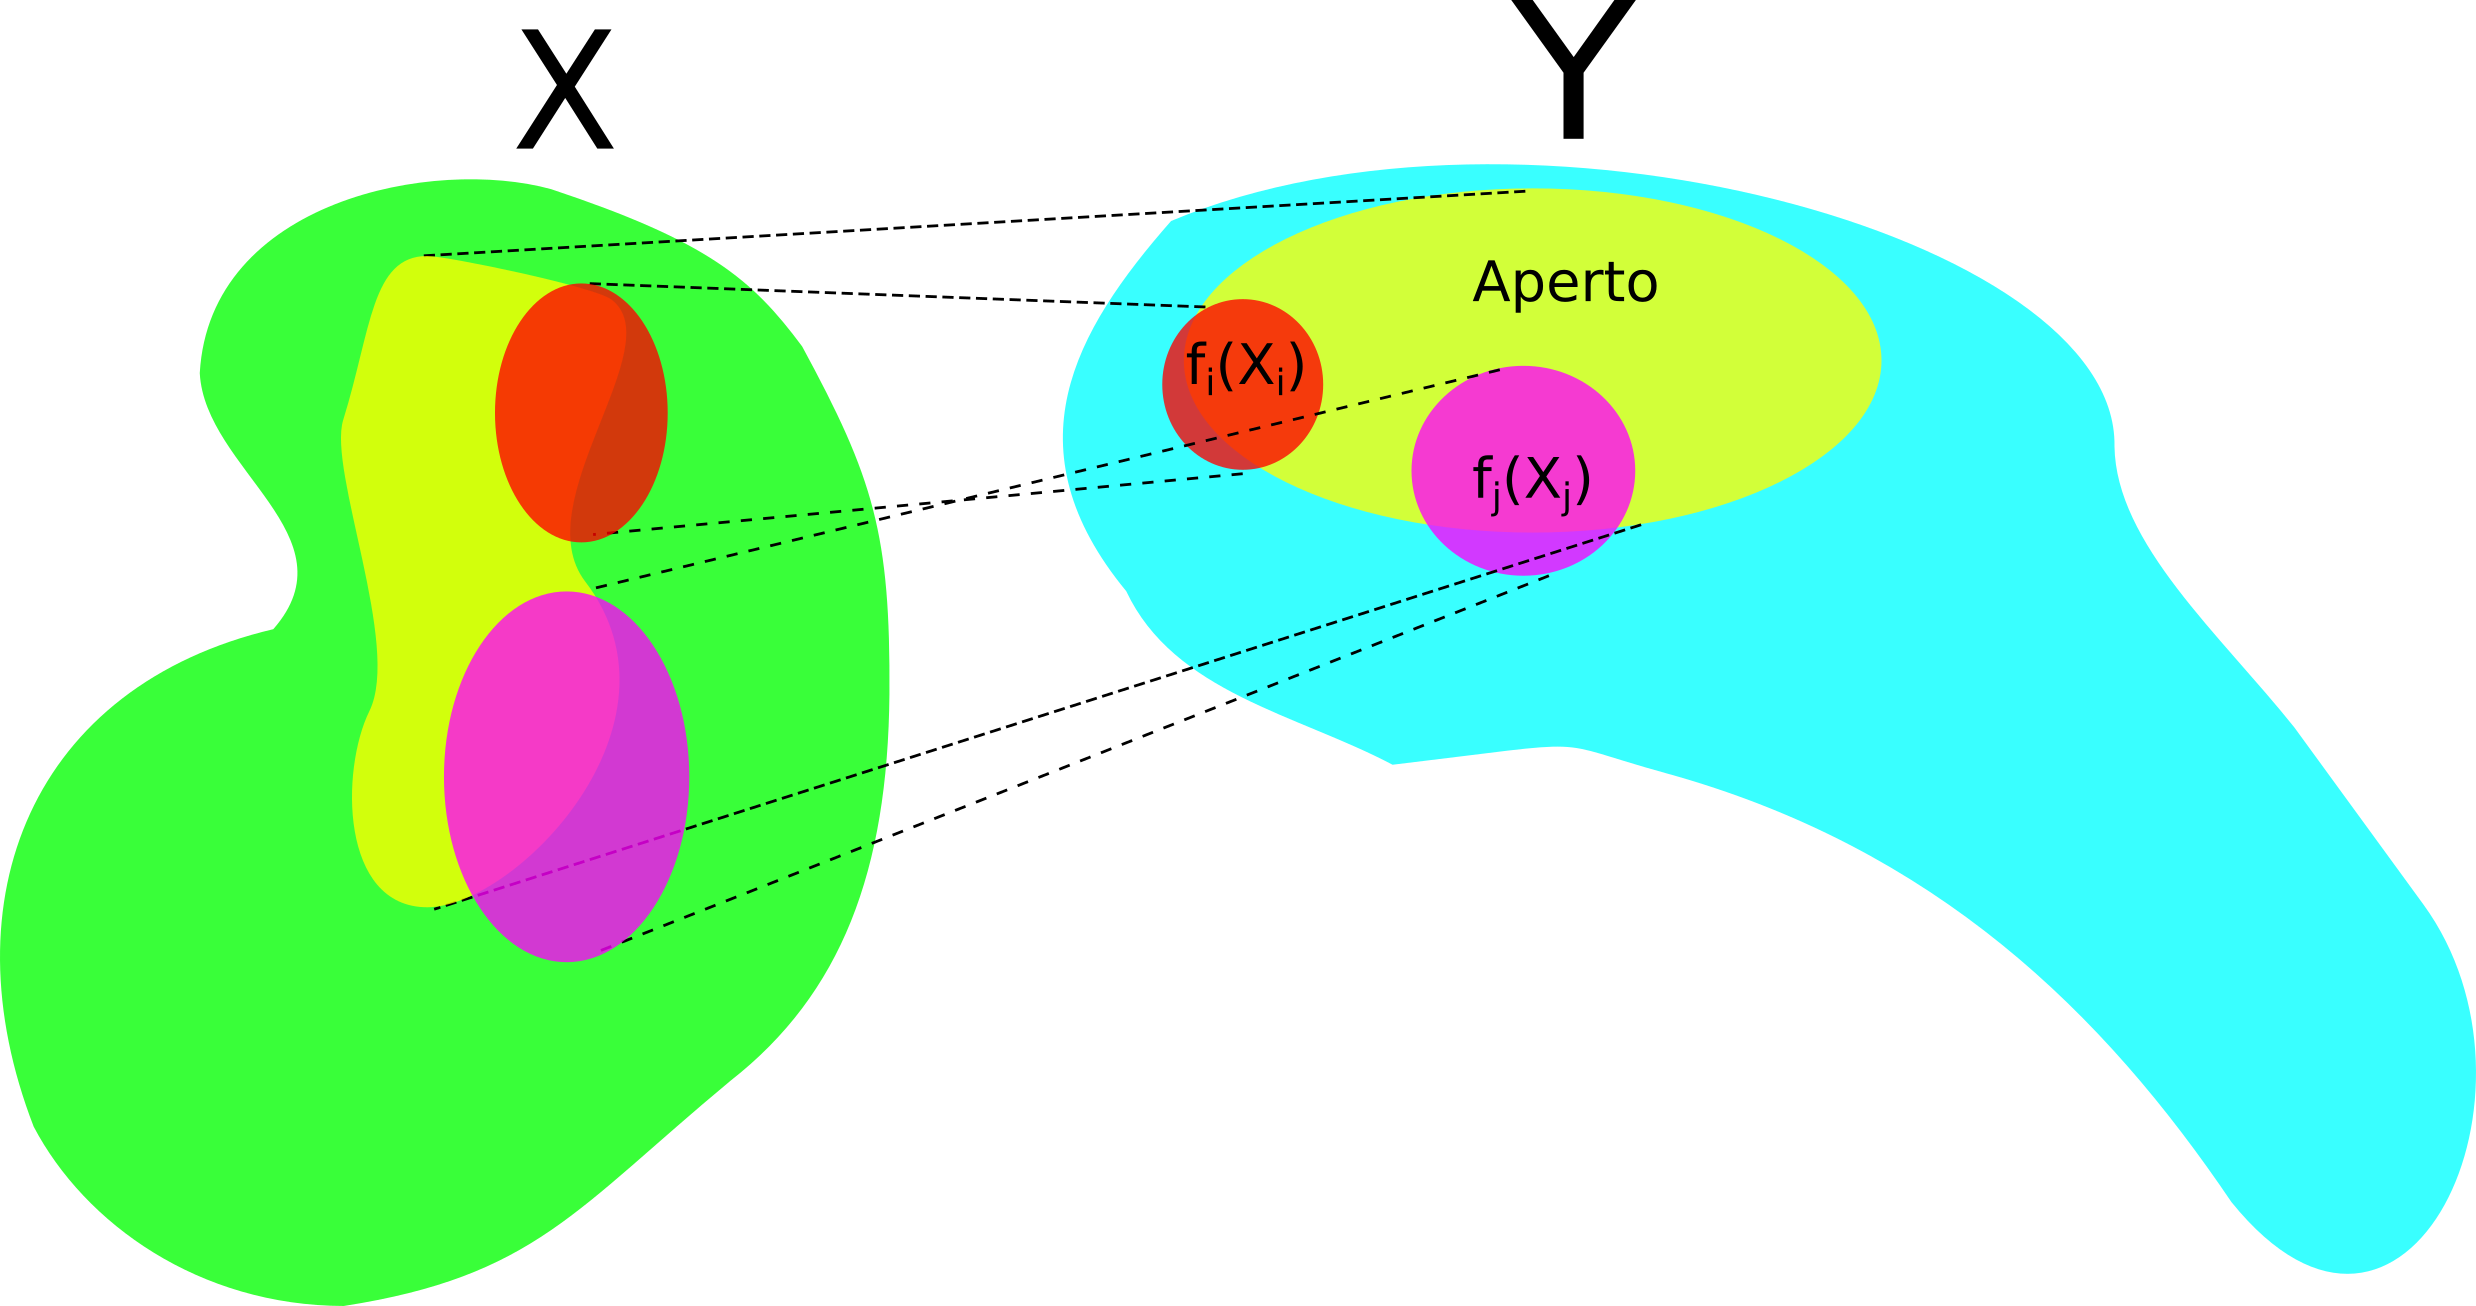
\includegraphics[width=0.6\linewidth]{images/topologia_generale/Coomology_exercises_figure}
		\caption{}
		\label{fig:coomologyexercisesfigure}
	\end{figure}

	Sia $A$ aperto in $\xi$. Allora considero $f^{-1}(A)$. Per la definizione di $f$ e siccome potrebbe essere che una parte di $A \cap \image{f_j} \neq \varnothing$ e $A \cap \image{f_i} \neq \varnothing$, allora prendo tutte quelle funzioni la cui immagine contiene punti di $A$. Allora vale 
	\begin{equation*}
		f^{-1}(A) = \bigcup_{i} f_i^{-1}(A) 
	\end{equation*}
	ma poiché $f_i$ è continua in $X_i$, dev'essere che $f^{-1}(A) = X_i \cap A_i'$ dove $A' \in \tau$. Dunque 
	\begin{equation*}
		f^{-1}(A) = \bigcup_{i} f_i^{-1}(A) = \bigcup_{i} X_i \cap A_i' 
	\end{equation*}
	ma $X_i, A'_i \in \tau$ quindi la loro intersezione è ancora un aperto, inoltre l'intersezione qualsiasi di aperti è un aperto. Segue che $f^{-1}(A)$ è aperto e dunque $f$ continua.
\end{proof}


\section{Prodotto di topologie}

In questa sezione si userà spesso la notazione $(X_1, \tau_1), (X_2, \tau_2), (X_1 \times X_2, \tau = \left\langle\tau_1 \times \tau_2 \right\rangle)$ per indicare tre spazi topologici. Quest'ultimo è il prodotto di due spazi topologici che adesso definiamo.

\begin{definition}
	La topologia $\tau$ che viene generata dalla base $\tau_1 \times \tau_2$ è detta topologia prodotto su $X_1 \times X_2$. Inoltre $(X_1 \times X_2, \tau)$ è uno spazio topologico e si dice prodotto degli spazi topologici $(X_1, \tau_1), (X_2, \tau_2)$.
\end{definition}

\begin{remark}
	Per quanto ovvio, facciamo vedere che $\tau_1 \times \tau_2$ forma una base su $X_1 \times X_2$. Per la Proposizione \ref{thr:sfi_generate_topology} un insieme è una base di $X_1 \times X_2$ se tale insieme copre $X_1 \times X_2$, ma questo è ovvio visto che $X_1 \times X_2 \in \tau_1 \times \tau_2$; e dati due elementi $A_1, A_2 \in \tau_1 \times \tau_2$ allora la loro intersezione $A_1 \cap A_2 = B_{1,1} \times B_{2,1} \cap B_{2,1} \times B_{2,2} = B_{1,1}\cap B_{2,1} \times B_{1,2} \cap B_{2,2}$ dove ogni $B_{j,i} \in \tau_j \cap A_i$ per cui sono ancora elementi di $\tau_1 \times \tau_2$. Pertanto è una base e identifica un unica topologia.
\end{remark}

\begin{example}
	Si consideri $(\R^2, \tau^2_{\text{euclidea}})$, questo sarà omeomorfo a $(\R, \tau) \times (\R, \tau)$? Se la risposta fosse negativa non avrebbe senso parlare di prodotti di topologie, pertanto la risposta dev'essere affermativa. 
	% TODO: `EASY PROOF: manca la dimostrazione \R^2 \simeq \R\times \R
	In generale quindi $\tau^n = \underset{n-volte}{\underbrace{\tau \times \dots \times \tau}}$ dove $\tau$ è la topologia euclidea. 
\end{example}

\begin{theorem}
	Sia $\mathcal{B}_1$ base di $\tau_1$ e $\mathcal{B_2}$ base di $\tau_2$, allora
	\begin{equation*}
		\mathcal{B}_1 \times \mathcal{B}_2 \coloneqq \left\{B_1 \times B_2 \in 2^{\mathcal{B}_1 \times \mathcal{B}_2} \,\middle|\, B_1 \in \mathcal{B}_1, \; B_2 \in \mathcal{B}_2\right\}
	\end{equation*}
	forma una base della topologia $\tau$ (ovvero il generato del prodotto delle topologie).
\end{theorem}
\begin{proof}
	Devo far vedere che se $A \in \tau$ allora è generato dalla base $\mathcal{B}_1 \times \mathcal{B}_2$. Allora se $A \in \tau$, la topologia è generata dalla base $\tau_1 \times \tau_2$. Per cui $A = \bigcup_{i \in I} A_{1,i} \times A_{2,i}$ dove $A_{1,i} \in \tau_1$ e $A_{2.i} \in \tau_2$ per ogni $i \in I$. Ma ogni $A_{1, i} = \bigcup_{B \in \mathcal{B}_{1,i}'} B$ dove $\mathcal{B}_{1,i}' \subset \mathcal{B}_1$ e analogamente per $A_{2,i}$. Sostituendo si ottiene
	\begin{equation*}
		A = \bigcup_{i \in I} A_{1,i} \times A_{2,i} = \bigcup_{i \in I} \bigcup_{B \in \mathcal{B}_{1,i}'} B \times \bigcup_{B \in \mathcal{B}_{2,i}'} B = \bigcup_{\substack{i \in I \\ B_1 \in \mathcal{B}'_{1,i} \\ B_2 \in \mathcal{B}'_{2,i}}} B_1 \times B_2
	\end{equation*}
	Notare che $B_1 \times B_2$ indica tutti i possibili prodotti tra gli insiemi nelle rispettive famiglie, $\mathcal{B}'_{1,i}$ e $\mathcal{B}'_{2,i}$, e questi sono sempre elementi di $\mathcal{B}_1 \times \mathcal{B}_2$ e la somma dipende solo da $I$, per cui genera $A$. \\
	
	Devo vedere anche che la topologia generata da $\mathcal{B}_1 \times \mathcal{B}_2$ non sia più fine di $\tau$. Per cui sia $A \in \left\langle \mathcal{B}_1 \times \mathcal{B}_2 \right\rangle$. Allora $A = \bigcup_{i \in I} B_{1,i} \times B_{2,i}$, mi basta considerare la proiezione di $A$ (che è una mappa aperta) per vedere che $\pi_1(A) = \bigcup_{i \in I} B_{1,i} = A_1 \in \tau_1$ e analogamente per $\tau_2$. Per cui risulta che $A_1 \times A_2 = \pi_1(A) \times \pi_2(A) = A$.
\end{proof}


\begin{theorem}
	La topologia prodotto $\tau$ è la meno fine per cui le mappe $\morphism{\pi_i}{X_1\times X_2}{X_i}$ sono continue.
\end{theorem}
\begin{proof}
	Suppongo esista una topologia meno fine di $\tau$ che chiamerò $\tau'$. Allora $\pi_1$ è continua e quindi contine almeno tutti gli aperti della forma $\pi^{-1}_1(A_1) \times \pi^{-1}_2(A_2)$ dove $A_i$ aperto in $\tau_i$. Ma questi aperti sono esattamente gli aperti della base che generano $\tau$, pertanto $\tau \subset \tau'$.
\end{proof}

\begin{theorem}
	Le mappe $\morphism{\pi_i}{X_1\times X_2}{X_i}$ sono aperte (dove $i \in \left\{1,2\right\}$). 
\end{theorem}
\begin{proof}
	Si consideri $\pi_1(A)$ dove $A \in \tau$. Allora $A = \bigcup_{i \in I} A_{1,i} \times A_{2,i}$, per cui $\pi(A) = \pi(\bigcup_{i \in I} A_{1,i} \times A_{2,i}) = \bigcup_{i\in I} \pi_1 (A_{1,i} \times A_{2,i}) = \bigcup_{i \in I} A_{1,i}$. Poiché ogni $A_{1,i} \in \tau_1$ segue che anche la loro unione lo è. Analogamente si dimostra per la proiezione $\pi_2$.
\end{proof}

\begin{theorem}
	Siano $S_1 \subset X_1, S_2, \subset X_2$ allora il prodotto di sottotopologie si comporta bene, ovvero
	\begin{equation*}
		\left\langle \tau_1 \times \tau_2 \right\rangle|_{S_1 \times S_2} = \left\langle \tau_1|_{S_1} \times \tau_2|_{S_2} \right\rangle 
	\end{equation*}
\end{theorem}
\begin{proof}
	Spezzo la dimostrazione nelle due inclusioni. Dimostro come primo caso $	\left\langle \tau_1 \times \tau_2 \right\rangle|_{S_1 \times S_2} \subset \left\langle \tau_1|_{S_1} \times \tau_2|_{S_2} \right\rangle$. Quindi sia $A \in \left\langle \tau_1 \times \tau_2 \right\rangle|_{S_1 \times S_2}$ allora $A = \left( \bigcup_{i \in I} A_{1,i} \times A_{2,i} \right) \cap S_1 \times S_2$, per cui posso distribuire l'intersezione su tutti gli elementi dell'unione:
	\begin{equation*}
		\left( \bigcup_{i \in I} A_{1,i} \times A_{2,i} \right) \cap S_1 \times S_2 = \bigcup_{i \in I} (A_{1,i} \cap S_1) \times (A_{2,i} \cap S_2)
	\end{equation*}
	per il Teorema \ref{thr:proprieties_induced_top} per ogni $i \in I$, $(A_{1,i} \cap S_1) \times (A_{2,i} \cap S_2) \in \tau_1|_{S_1} \times \tau_2|_{S_2}$, ovvero $A \in \left\langle \tau_1|_{S_1} \times \tau_2|_{S_2} \right\rangle$. Come si può notare le implicazioni fatte sopra valgono anche nel verso opposto, per cui è dimostrata la tesi.
\end{proof}

\begin{theorem}
	Gli intorni si \emph{comportano bene} rispetto al prodotto topologico. In particolare
	\begin{enumerate}
		\item Sia $(x_1, x_2) \in X_1\times X_2$. Allora $P \in \mathcal{N}_\tau((x_1,x_2))$ se e solo se esitono $U_1 \in \mathcal{N}_{\tau_1}(x_1)$ e $U_2 \in \mathcal{N}_{\tau_2}(x_2)$ tali che $U_1\times U_2 \subset P$.
		\item Sia $(x_1, x_2) \in X_1\times X_2$, $\mathcal{V}_1(x_1)$ e $\mathcal{V}_2(x_2)$ rispettivamente un sistema fondamentale di intorni di $x_1$ in $\tau_1$ e di $x_2$ in $\tau_2$. Allora $\mathcal{V}_1(x_1) \times \mathcal{V}_2(x_2)$ è un sistema fondamentale di intorni di $(x_1, x_2)$ nella topologia $\tau = \left\langle \tau_1 \times \tau_2 \right\rangle$.
	\end{enumerate}	
\end{theorem}
\begin{proof}[Punto 1]
	\begin{enumerate}
		\item[$\Leftarrow$] Abbastanza ovvio. Per definizion di intorno su $U_1$, allora esiste $A_1 \in \tau_1$ tale che $A_1 \subset U_1$ e analogo discorso su $\tau_2$. Per cui $A_1 \times A_2 \in \tau$ per definizione, inoltre ho che 
		\begin{equation*}
			A_1 \times A_2 \subset U_1 \times U_2 \subset P
		\end{equation*}
		per cui $P$ è un intorno in $\tau$.
		\item[$\Rightarrow$] Per definizione di intorno vuol dire che esiste $A \subset P$ tale che $A \in \tau$. Allora $A = \bigcup_{i \in I} A_{1,i} \times A_{2,i}$, prendo $A_{1,i_0}, A_{2,i_0}$ tali da contenere rispettivamente $x_1, x_2$. Devo dimostrare che $A_{1,i_0}$ è un intorno di $x_1$ in $\tau_1$, ma è ovvio poiché $A_{1,i_0} \in \tau_1$. Analogo discorso su $A_{2,i_0}$. Ho dunque trovato un intorno in $\tau_1$ e uno in $\tau_2$ tali che il loro prodotto sta in $P$ (poiché il loro prodotto sta addirittura in $A \subset P$).
	\end{enumerate}
\end{proof}
\begin{proof}[Punto 2]
	% TODO: `EASY PROOF': Dimostrazione che gli intorni si comportano bene nel prodotto topologico.
\end{proof}

\begin{theorem}
	Siano $S_1 \subset X_1, S_2 \subset X_2$, allora valgono le seguenti formule
	\begin{align}
		\overline{S_1\times S_2}^{\tau} & = \overline{S_1}^{\tau_1} \times \overline{S_2}^{\tau_2} \\
		Int(S_1 \times S_2) & = Int(S_1) \times Int(S_2)\\
		Fr(S_1 \times S_2) &= (Fr(S_1) \times \overline{S_2}) \cup (\overline{S_1} \times Fr(S_2))
	\end{align}
\end{theorem}
\begin{proof}[Dimostrazione equazione 1]
	Uso il fatto che un punto $x \in \overline{S_1\times S_2}^\tau$ se e solo se $x$ è aderente a $S_1 \times S_2$ in $\tau$. Fisso dunque un $(x_1, x_2) \in \overline{S_1\times S_2}^\tau$ e dei sistemi fondamentali di intorni $\mathcal{V}_{\tau_1}(x_1), \mathcal{V}_{\tau_2}(x_2)$.\\
	L'aderenza per definizione vuol dire che esiste un sistema fondamentale di intorni $\mathcal{V}_\tau(x) = \mathcal{V}_{\tau_1}(x_1) \times \mathcal{V}_{\tau_2}(x_2)$ tale che per ogni $V \in \mathcal{V}_\tau(x)$ vale $V \cap S_1 \times S_2 \neq \varnothing$. Usando la definizione data di $\mathcal{V}_\tau(x)$ posso riscrivere come per ogni $V_1 \in \mathcal{V}_{\tau_1}(x_1), V_2 \in \mathcal{V}_{\tau_2}(x_2)$ tali che $V_1 \times V_2 \cap S_1 \times S_2 \neq \varnothing$. \\
	Applicando un po' di leggi insiemistiche diventa $V_1 \cap S_1 \times V_2 \cap S_2 \neq \varnothing$, ovvero $V_1 \cap S_1 \neq \varnothing$ e $V_2 \cap S_2\neq \varnothing$ per cui dev'essere che $x_1$ sia aderente a $S_1$ secondo $\tau_1$ e analogamente per $x_2$. Per cui vale l'equazione. 
\end{proof}
\begin{proof}[Dimostrazione equazione 2]
	% TODO: `EASY PROOF': Dimostrare che Int(S × T) = Int(S) × Int(T)
\end{proof}
\begin{proof}[Dimostrazione equazione 3]
	Considero, analogamente a quanto fatto per dimostrare la prima equazione, posso prendere $(x_1,x_2) \in Fr(S_1 \times S_2)$. Fisso un sistema fondamentale di intorni su $S_1$ e $S_2$. Per cui se $x \in Fr(S_1 \times S_2)$ allora $V \cap S_1 \times S_2\neq \varnothing$ e $V \not\subset S_1 \times S_2$. Sostituendo la decomposizione per sistemi fondamentali di intorni $V_1 \times V_2 \cap S_1 \times S_2 = V_1 \cap V_2 \times S_1 \cap S_2\neq \varnothing$ per cui $V_1 \cap S_1 \neq \varnothing$ e $V_2 \cap S_2 \neq \varnothing$. Inoltre dalla condizione $V \not\subset S_1 \times S_2$ si ottiene le tre condizione $V_1 \subset S_1 \land V_2 \not\subset S_2$ o $V_1 \not\subset S_1 \land V_2 \subset S_2$ o $V_1 \not\subset S_1 \land V_2 \not\subset S_2$. Unendo tutte le condizioni si ottiene la tesi. 
\end{proof}

\begin{theorem}[Proprientà universale del prodotto topologico]
	\begin{equation*}
		\begin{tikzcd}[column sep=0.7em]
		& (Y, \xi) \arrow[swap]{d}{f} \arrow[swap]{ddl}{f_1} \arrow{ddr}{f_2} & \\
		& (X_1 \times X_2, \tau) \arrow[swap]{dr}{\pi_2} \arrow{dl}{\pi_1} & \\
		(X_1, \tau_1) &  & (X_2, \tau_2)\\
		\end{tikzcd}
	\end{equation*}
	Sia $\morphism{f}{(Y, \xi)}{(X_1 \times X_2, \tau)}$ una applicazione su spazi topologici e siano $\pi_1,\pi_2$ le proiezioni canoniche dal prodotto topologico. Allora $f_i = \pi_i \circ f$ si dicono componenti di $f$ e vale l'equivalenza delle seguenti affermazioni:
	\begin{enumerate}
		\item $f$ è continua;
		\item $f_i$ sono continue per $i \in \left\{1,2\right\}$.
	\end{enumerate}
\end{theorem}
\begin{proof}[Dimostrazione 1]
	\begin{enumerate}
		\item[$\Leftarrow$] Se $f$ continua allora $\pi_1 \circ f$ è continua perché composizione di funzioni continue, analogamente per $\pi_2 \circ f$.
		\item[$\Rightarrow$] Se le componenti $f_1, f_2$ sono continue. Allora si prenda un aperto $A \in \tau$, e si prenda la sua controimmagine attraverso $f$. È ovvio che 
		\begin{equation*}
			f^{-1}(A) = f^{-1}(\bigcup_{i \in I} A_{1,i} \times A_{2,i}) = \bigcup_{i \in I} f^{-1}(A_{1,i} \times A_{2,i})
		\end{equation*}
		dove $A_{1,i}, A_{2,i}$ sono aperti rispettivamente in $\tau_1, \tau_2$. Siccome non abbiamo ancora usato l'ipotesi, è arrivato il momento di usarla. Infatti si vede che $f^{-1}_1(A_{1,i}) \cap f^{-1}_2(A_{2,i}) = f^{-1}(A_{1,i} \times A_{2,i})$, ma essendo $f_1, f_2$ continue, la loro controimmagine di aperti è aperta. Da cui ho anche $f^{-1}(A_{1,i} \times A_{2,i})$ aperto. Per cui $f$ è continua. 
	\end{enumerate}
\end{proof}
\begin{proof}[Dimostrazione utilizzando le proprietà degli s.f.i.]
	% TODO: `? CASUAL': Una dimostrazione alternativa, di un teorema già dimostrato
\end{proof}

\begin{theorem}
	Sia $\morphism{g}{(X_1 \times X_2, \tau)}{(Y, \xi)}$. Fissato un $(x_1, x_2) \in X_1 \times X_2$. Allora posso dire che $g$ è continua in $(x_1, x_2)$ se per ogni $U \in \mathcal{N}_\xi(g(x_1,x_2)))$ esistono $V_1 \in \mathcal{V}_1(x_1)$ e $V_2 \in \mathcal{V}_2(x_2)$ tali che $g(V_1 \times V_2) \subset U$.
\end{theorem}
\begin{proof}
	Se $g$ è continua in $x$ allora per ogni intorno $V$ di $g(x)$ esisterà un intorno $N$ di $x$ tale che $g(N) \subset V$. Poiché $N$ è un intorno nella topologia prodotto allora esistono $N_1, N_2$ rispettivamente intorni di $x_1, x_2$ dove $x = (x_1, x_2)$. Ovvero la tesi.\\
	Al contrario fissiamo un $V$ intorno di $g(x)$, allora devo dimostrare che $g^{-1}(V)$ è ancora un intorno di $x$, ma questo è ovvio dato che esistono $N_1, N_2$ tali che $g(N_1 \times N_2) \subset g(g^{-1}(V)) \subset V$ e quindi $N_1 \times N_2 \subset g^{-1}(V)$. 
\end{proof}

Notare che in generale i teoremi dimostrati per $n=2$, ovvero $X_1 \times X_2$, valgono anche per $n \in \N$, infatti basta procedere per induzione. Il vero problema è dimostrare che $X_1 \times X_2 \times \dots \times X_n \simeq X_1 \times (X_2 \times \dots \times X_n)$ e così via. Ovvero dimostrare che il prodotto di topologie è un operatore associativo nella categoria degli spazi topologici. 

\begin{theorem}
	Le topologie con il prodotto formano un monoide commutativo su $\mathbb{Top}/\sim$ dove $X\sim Y$ se e solo se $X$ è omeomorfo $Y$.
\end{theorem}
\begin{proof}
	\begin{enumerate}
		\item Associatività. 
		\item Commutatività. Basta definire la mappa $\morphism{f}{X\times Y}{Y \times X}$, con $f(x,y) = (y,x)$. La mappa così definita è continua, biettiva e aperta. Per cui la commutatività vale.
		\item L'identita è il singoletto $\left\{p\right\}$ con la topologia qualsiasi (tanto è sempre la solita). Quindi sia $(X, \tau)$ uno spazio topologico. Definisco la mappa $\morphism{f}{(X, \tau)}{(X\times \left\{p\right\}, \tau'}$ definibile nell'unico modo possibile. La mappa è biettiva perché $f^{-1}(x, p) = x$ è la sua funzione inversa. È ovviamente continua perché $f^{-1}((A, \varnothing)) = \varnothing$, $f^{-1}((A, \left\{p\right\})= A$ perché $f$ biettiva. E analogamente si dimostra che è aperta. Pertanto è l'identità. 
	\end{enumerate}
\end{proof}

\section{Topologie quozienti}

\begin{definition}[Topologia quoziente]
	Sia $(X, \tau)$ spazio topologico e $\morphism{f}{X}{Y}$ applicazione, con $Y \neq \varnothing$. Si dice topologia quoziente su $Y$ rispetto ad $f$, oppure topologia indotta da $f$ su $Y$, la più fine topologia su $Y$ tale che $f$ è continua. 
\end{definition}

\begin{theorem}
	Sia $(X, \tau)$ spazio topologico e $\morphism{f}{X}{Y}$ applicazione e $Y \neq \varnothing$. Valgono le seguenti affermazioni 
	\begin{enumerate}
		\item La topologia quoziente su $Y$ rispetto a $f$ esiste ed è unica, denotandola come $\tau_f$ vale 
		\begin{equation*}
			\tau_f \coloneqq \left\{ A \in 2^Y \,\middle|\, f^{-1}(A) \right\}
		\end{equation*}
		\item $C$ è chiuso in $\tau_f$ se e solo se $f^{-1}(C)$ è chiuso in $\tau$.
		\item \textbf{Proprietà universale degli  spazi quozienti} 
		\begin{equation*}
		\begin{tikzcd}
		(X, \tau) \arrow[swap]{rd}{g\circ f} \arrow{r}{f} & (Y, \tau_f) \arrow{d}{g} \\
		& (Z, \mu) 
		\end{tikzcd}
		\end{equation*}
		$g$ è continua se e solo se $g \circ f$ è continua. 
	\end{enumerate}
\end{theorem}
\begin{proof}
	\begin{enumerate}
		\item È ovviamente una topologia ed è la più fine. 
		\item La controimmagine commuta con il complementare. 
		\item Se $g$ è continua è ovvio che $g \circ f$ è continua perché la composizione di funzioni continue è continua. Se $f\circ g$ è continua allora se $g$ continua allora $g^{-1}(A)$ è un aperto. Ma $ \tau_f \ni g^{-1}(A) \Leftrightarrow f^{-1}g^{-1}(A) \in \tau$ ma l'ultima è banalmente ovvia visto che $g \circ f$ continua. \footnote{Perché è interessante questa proprietà universale? Innanzitutto perché è universale su tutte le topologie quozienti, secondariamente perché ti permette di by-passare la topologia quoziente per trovare che una mappa è continua, senza dover lavorare sulla topologia quoziente stessa.}
	\end{enumerate}
\end{proof}

\begin{remark}
	sia $\morphism{f}{(X, \tau)}{Y, \tau_f)}$ se $f$ non surgettiva allora $\exists y \in Y \setminus f(X)$, il singoletto $\left\{y\right\}$ è un aperto nella topologia $\tau_f$ poiché $f^{-1}(y) = \varnothing$.
\end{remark} 

\begin{definition}
	Sia $\morphism{f}{X}{Y}$ applicazione e sia $S \subset X$. Diciamo che $S$ è \textbf{saturo}\footnote{Un'idea del termine è che essenzialmente la funzione \textit{divora} tutte le fibre di $S$ in modo tale che stiano in $S$ stesso, infatti se ho una saturazione ho la stessa cosa} rispetto a $f$, se $f^{-1}(f(S)) = S$.
\end{definition} 

\begin{remark}
	$S$ è saturo in $f$.
	\begin{equation*}
		S = f^{-1}f(S) = \bigcup_{x \in S} f^{-1}f(x)
	\end{equation*}
	ovvero se per ogni $x \in S$ abbiamo una unica fibra in $S$. Ovvero $S$ contiene tutte le fibre contenenti i suoi punti. 
\end{remark} 

\begin{remark}
	Se $f$ iniettiva allora ogni insieme è $f$-saturo, poiché $S = f^{-1}f(S)$.
\end{remark}

\begin{theorem}
	$\morphism{f}{X}{Y}$ applicazione e sia $S \subset X$. $f^{-1}f(S)$ si dice \textbf{$f$-saturazione} di $S$. Si può dimostrare che 
	\begin{enumerate}
		\item $S \subset f^{-1}f(S)$
		\item $f^{-1}f(S)$ è il più piccolo insieme $f$-saturo contenente $S$.
	\end{enumerate}
\end{theorem}
\begin{proof}
	\begin{enumerate}
		\item Ovvio. Volendo usare quanto detto nell'osservazione precedente
		\begin{equation*}
			S = \bigcup_{x\in S} \left\{x\right\} \subset \bigcup_{x \in S} f^{-1}f(x)
		\end{equation*}
		\item È semplice vedere che
		\begin{equation*}
			f(f^{-1}(f(S))) = f(S) \Longrightarrow f^{-1}(f(f^{-1}(f(S)))) = f^{-1}(f(S))
		\end{equation*}
		poiché se $x \in f^{-1}(f(S))$ allora $f(x) \in f(S)$ per definizione (e viceversa), quindi la $f$-saturazione di $S$ è $f$-satura. Devo inoltre dimostrare che è la più piccola. Per cui sia $K$ $f$-saturo tale che $S \subset K \subset f^{-1}f(S)$. Allora applicando $f^{-1}f$ sulla precedente successione di inclusioni
		\begin{equation*}
			f^{-1}f(S) \subset f^{-1}f(K) \overset{\text{è f-sat.}}{=} K \subset f^{-1}ff^{-1}f(S) = f^{-1}f(S) 
		\end{equation*}
		per cui dev'essere che $K = f^{-1}f(S)$. Per cui la più piccola è per forza $f^{-1}f(S)$ 
	\end{enumerate}
\end{proof}


\section{Quozienti con mappe surgettive}

Poiché la topologia quoziente è difficile da studiare da sola, quindi si  cerca di collegare le proprietà della topologia $\tau_f$ a quella di partenza $\tau$.

\begin{lemma}
	$\morphism{f}{X}{Y}$ applicazione surgettiva e $S \subset X$ $f$-saturo, allora 
	\begin{enumerate}
		\item $S^c$ è $f$-saturo 
		\item $f(S^c) = f(S)^c$
	\end{enumerate}
\end{lemma}
\begin{proof}
	Dimostro per prima cosa $f(S)^c = f(S^c)$. Data $f$ suriettiva allora 
	\begin{equation*}
		f(X) = f(S \cup S^c) = f(S) \cup f(S^c) = Y
	\end{equation*}
	e dunque $f(S^c) = Y \setminus f(S) = f(S)^c$. 
	Per la $f$-saturazione di $S$ ho che $S = f^{-1}f(S)$, dunque applicando il complementare ho che $S^c = f^{-1}(f(S))^c = f^{-1}(f(S)^c) = f^{-1}(f(S^c))$
\end{proof}

\begin{theorem}
	Sia $(X, \tau)$ spazio topologico e $\morphism{f}{X}{Y}$ surgettiva e dato $Y$ con $\tau_f$ allora vale 
	\begin{enumerate}
		\item $A \subset Y$ è un aperto in $\tau_f$ se e solo se esiste $Q \in \tau$ tale da essere $f$-saturo e che $f(Q) = A$. Dunque vale 
		\begin{equation*}
			\tau_f = \mathcal{A} = \left\{ A \in 2^Y \,\middle|\, A = f(S), \text{dove}\ S \in \tau, f^{-1}f(S) = S\right\}
		\end{equation*}
		\item $C \subset Y$ è un chiuso in $\tau_f$ se e solo se esiste $Q \subset X$ chiuso tale da essere $f$-saturo e che $f(Q) = C$.
	\end{enumerate}
\end{theorem}
\begin{proof}
	\begin{enumerate}
			\item Sia $A \in \mathcal{A}$ allora esiste $S \in \tau$ tale da essere $f$-saturo. Per cui $f^{-1}(A) = f^{-1}(f(S)) \overset{\text{saturazione}}{=} S \in \tau$. Questo dimostra $\mathcal{A} \subset \tau_f$. Sia dunque $A \in \tau_f$ e $U = f^{-1}(A) \in \tau$ devo dimostrare che $U$ è $f$-saturo. 
			Dato che $f(f^{-1}(A)) = A$ per la surgettività di $f$   
			\begin{equation*}
				f^{-1}f(U) = f^{-1}(A) = U
			\end{equation*} 
			e dunque è anche $f$-saturo. Si evince che $\tau_f \subset \mathcal{A}$ e dunque anche che $\tau_f = \mathcal{A}$.
		\item Devo dimostrare che un chiuso in $\tau_f$ è sempre della forma $K = f(C)$ per $C$ $f$-saturo e $C$ chiuso in $\tau$. Quindi vale che $K^c = f(S)$ dove $S \in \tau$ e $f$-saturo. Quindi posso riscrivere $S = C^c$ dove $C$ chiuso in $\tau$. Per il precedente lemma ho dunque
		\begin{equation*}
			K^c = f(S) = f(C^c) \overset{\text{lem. prec.}}{=} f(C)^c
		\end{equation*}
		dove $C$ è un chiuso $f$-saturo. Ovvero per ogni $K$ chiuso in $\tau_f$, vale $K = f(C)$ per qualche $C$ chiuso in $\tau$ e $f$-saturo (e viceversa), cioè la tesi.
	\end{enumerate}
\end{proof}

\begin{definition}
	Una applicazione $\morphism{f}{(X,\tau)}{(Y, \xi)}$ tra spazi topologici è detta \textbf{identificazione} se $f$ è continua, surgettiva e $\xi = \tau_f$.
\end{definition}

\begin{theorem}[Caratterizzazione delle indentificazioni]
	\label{crtident}
	Sia $\morphism{f}{(X,\tau)}{(Y, \xi)}$ applicazione continua e surgettiva, allora le seguenti affermazioni sono equivalenti
	\begin{enumerate}
		\item $f$ è un identificazione
		\item Se $\forall A \subset Y$  tale che $f^{-1}(A) \in \tau$ allora $A \in \xi$
		\item Se $\forall A \in \tau$, $A$ è $f$-saturo e $f(A) \in \xi$.
		\item Se $\forall C \subset X$ chiuso e $f$-saturo vale $f(C)$ chiuso in $\xi$
	\end{enumerate}
\end{theorem}
\begin{proof}
	\begin{enumerate}
		\item[$1 \Leftrightarrow 2$] $f$ identificazione se e solo se $\tau_f = \xi$ e abbiamo gratis che $\xi \subset \tau_f$ perché topologia più fine tale da render $f$ continua. Quindi bisogna dimostrare $\tau_f \subset \xi \Longleftrightarrow \forall A \subset Y$ tali che $f^{-1}(A) \in \tau \Rightarrow A \in \xi$. Per cui se vale $\tau_f \subset \xi$ è ovvio che ogni $A$ $f^{-1}(A) \in \tau$ allora $A \in \tau_f \subset \xi$ e ho la tesi. Se invece vale $\forall A \subset Y$ tali che $f^{-1}(A) \in \tau \Rightarrow A \in \xi$ allora se prendo $A \in \tau_f$ allora dev'essere che $f^{-1}(A) \in \tau$ e per ipotesi vale anche che $A \in \xi$ quindi $\tau_f \subset \xi$. 
		\item[$1 \Rightarrow 3$] Fisso $U \in \tau$ tale da essere $f$-saturo, allora $f(U) \in \xi = \tau_f$, ma $\xi = \tau_f$ per ipotesi, ovvero si ottiene la tesi.
		\item[$3 \Rightarrow 1$] Se vale $f(U) \in \xi$ devo provare che $\xi = \tau_f$, ma $\xi \subset \tau_f$ è già dimostrata poiché $\tau_f$ è la topologia più fine per cui $f$ sia continua. Per cui fisso un $A \in \tau_f$. $A \in \tau_f \Leftrightarrow \exists U \in \tau$ e $f$-saturo, ma per ipotesi $f(U) \in \xi$, quindi $\tau_f \subset \xi \subset \tau_f$.
		\item[$3\Leftrightarrow 4$] Ovvio per teoremi precedenti.
	\end{enumerate}
\end{proof}


\begin{remark}
	Notare che le identificazioni nono sono sempre applicazioni aperte, anche se sono aperte e chiuse rispetto a una classe di insiemi (ovvero quelli $f$-saturi). Infatti possiamo definire una applicazione non aperta e non chiusa che chiamiamo $f$. Allora $\morphism{f}{(\R, \tau_{\text{euclidea}})}{(\left\{0,1\right\})}$, con $f \coloneqq \mathcal{X}_{\left[0,2\right)}$ dove la $\mathcal{X}$ è la mappa caratteristica dell'insieme a pedice. È ovvio che $\tau_f$ in questo caso è la topologia banale, infatti $0$ non può essere un aperto, in quanto se lo fosse $f^{-1}(0) = \left[0, 2\right)^c$ che non  è né aperto né chiuso. Analogamente per il punto $1$ che non può essere aperto (e neanche chiuso). Inoltre $f((0,2)) = 1$, per cui non manda aperti in aperti e analogamente si vede che $f(\left[0,1\right]) = 1$ e dunque non manda neanche chiusi in chiusi, eppure $f$ è una identificazione.
\end{remark}

\begin{theorem}
	Sia $\morphism{f}{(X,\tau)}{(Y, \tau_f)}$ identificazione allora valgono le seguenti affermazioni
	\begin{enumerate}
		\item $f$ aperta se e solo se $\forall A \in \tau$ la sua $f$-saturazione $f^{-1}f(A) \in \tau$
		\item $f$ chiusa se e solo se $\forall C$ chiuso la sua $f$-saturazione $f^{-1}f(C)$ è un chiuso.
	\end{enumerate}
\end{theorem}
\begin{proof}
	Dimostro solo il primo caso, il secondo è equivalente al primo dato quanto visto fin ora. Se $f$ aperta allora $\forall A \in \tau$ risulta che $f(A)$ è aperta per ipotesi e $f^{-1}f(A)$ dev'essere ancora un aperto perché $f$ continua. Se invece vale che la $f$-saturazione di un aperto è ancora aperta, fisso $A \in \tau$ e voglio vedere che $f(A)$ è un aperto in $\tau_f$. Ma $f(A) \in \tau_f$ se e solo se esiste $S \in \tau$ e $f$-saturo tale che $f(S) = f(A)$. Basta scegliere $S = f^{-1}f(A)$ e sappiamo che appartiene a $\tau$, è $f$-saturo e inoltre poiché $f$ suriettiva $f(S) = f(f^{-1}f(A)) = f(A)$. Pertanto $f$ è aperta. 
\end{proof}

\section{Relazioni di equivalenza e spazi quozienti}

Per creare uno spazio quoziente ci servono un paio di ingredienti
\begin{enumerate}
	\item Un insieme non vuoto, $X$.
	\item Una relazione di equivalenza $R \subset X \times X$.
\end{enumerate}

Una volta presi questi ingredienti è bene controllare le date di scadenza. Da qui in avanti diventa semplice, si quozientizza. Si prenda $X$ e lo si faccia diventare $X / R$ ovvero l'insieme delle classi di equivalenza di $X$ in $R$. 

\begin{figure}[h]
	\centering
	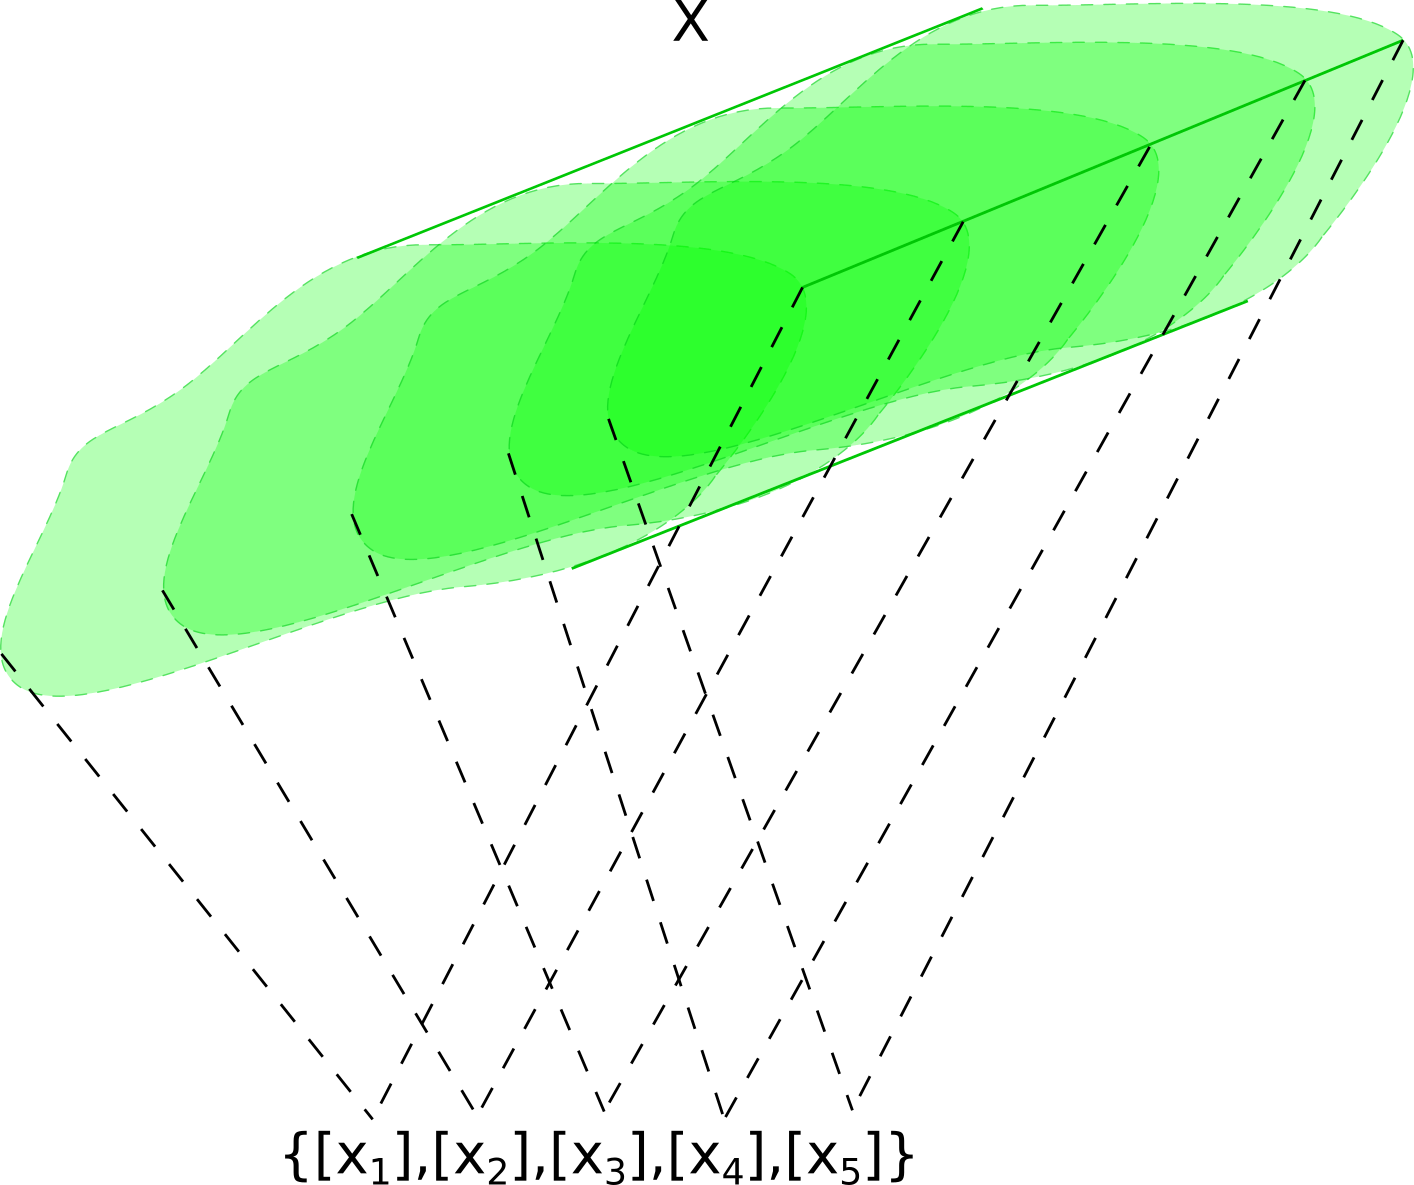
\includegraphics[width=0.5\linewidth]{images/topologia_generale/projection_quotient}
	\caption{Proiezione della partizione di $X$ data dalla relazione $R$. Oppure si possono vedere i sottoinsiemi verdi di $X$ come tutte le fibre di $f$ su un $X'$ e che vengono proiettate in un punto da $\pi$}
	\label{fig:projectionquotient}
\end{figure}

Dopo questo procedimento (circa 2-3 minuti) si può iniziare a operare sui morfismi e construire una mappa 
\begin{equation*}
\begin{tikzcd}[row sep = tiny]
	\pi  \colon &  X \arrow{r} & X/R \\
		 & x \arrow[mapsto]{r} & \left[x\right]_R
\end{tikzcd}
\end{equation*}


che è la \textbf{proiezione naturale} dell'insieme sul suo quoziente. Questa è sempre suriettiva (per questo si sono sempre studiate mappe suriettive nel capitolo precedente) e si comporta bene come si può vedere dalla figura. Utilizzando il procedimento canonico per la costruzione di topologie quozienti indotte da applicaizioni sulla proiezione naturale si ottiene quella che è detta \textbf{topologia quoziente di $\tau$ modulo $R$} e $(X/R, \tau_\pi)$ è detto lo spazio topologico quoziente di $(X,\tau)$ modulo $R$.

\begin{lemma}
	\label{lem_qdom}
	Sia $\morphism{f}{(X, \tau)}{(X', \tau')}$ applicazione continua tra spazi topologici e siano $R, R'$ relazioni di equivalenza rispettivamente su $X, X'$. Vale $f(\left[x\right]_R) \subset \left[f(x)\right]_{R'}$ (equivale alla condizione $xRy \Rightarrow f(x)R'f(y)$) se e solo se esiste ed è unica una $g$ continua tale che 
	\begin{equation*}
	\begin{tikzcd}[row sep = 3em]
		(X, \tau) \arrow[swap]{d}{\pi} \arrow{r}{f} & (X', \tau') \arrow{d}{\pi'}\\
		(X/R, \tau_{X/R}) \arrow[swap]{r}{\exists! g} & (X'/R', \tau_{X'/R'})
	\end{tikzcd}
	\end{equation*} 	
	il diagramma commuta.
\end{lemma}
\begin{proof}
	Se esiste $g$ per cui il diagramma commuta stiamo praticamente dicendo 
	\begin{equation*}
		(\pi' \circ f)(x) = (g \circ \pi)(x) = (g \circ \pi)(y) = (\pi' \circ f)(y)
	\end{equation*}
	ma questa uguaglianza vale se e solo se $f(x) R' f(y)$, per cui ho la tesi.\\
	
	Dimostro l'esistenza di $g$ e la definisco come $g(\alpha) = (\pi' \circ f)(x_\alpha)$ dove $x_\alpha = \pi^{-1}\alpha$, ovvero $x_\alpha$ è un rappresentante della classe $\alpha$. Devo far vedere che sia ben definita, altrimenti non \textit{esiste}.
	Per cui considero anche un altro rappresentate della classe $\alpha$ e lo chiamo $x'_\alpha$. Affinché sia ben definita dev'essere che $g(\alpha) = \pi'f(x_\alpha) = \pi' f(x'_\alpha) = g(\alpha)$, ma questa condizione è vera per l'ipotesi. La continuità di $g$ è data dalla proprietà universale degli spazi quozienti, si consideri il seguente diagramma commutativo
	\begin{equation*}
		\begin{tikzcd}[row sep = 3em]
			(X,\tau) \arrow{d}{\pi} \arrow{rd}{\pi' \circ f} & \\
			(X/R, \tau_{X/R}) \arrow{r}{g} & (X'/R', \tau_{X'/R'})
		\end{tikzcd}
	\end{equation*}
	per cui $g$ è continua dato che $\pi' \circ f$ è continua.
\end{proof}

\begin{theorem}
	Sia  $\morphism{f}{X}{X'}$ una applicazione continua e surgettiva possiamo definire la relazione di equivalenza $R_f$ sull'insieme $X$ ponendo la relazione $xR_fy \Leftrightarrow f(x) = f(y)$. Allora 
	\begin{enumerate}
		\item esiste ed è unica $\morphism{g}{X/R_f}{X'}$ tale che $g$ biettiva e continua.
		\item $g$ è un omeomorfismo se e solo se $f$ è un identificazione.
	\end{enumerate}
\end{theorem}
\begin{proof}
	Basta applicare il Lemma \ref{lem_qdom} sul seguente diagramma
	\begin{equation*}
	\begin{tikzcd}[row sep = 3em]
		(X, \tau) \arrow[swap]{d}{\pi} \arrow{r}{f} & (X', \tau') \arrow{d}{\pi' = \operatorname{Id}}\\
		(X/R_f, \tau_{X/R_f}) \arrow[swap]{r}{\exists! g} & (X'/U', \tau_{X'/U'}) = (X', \tau')
	\end{tikzcd}	
	\end{equation*}
	dove la relazione $U'$ su $X'$ è definita come $xU'y \Leftrightarrow x = y$, per cui la proiezione $\pi'$ non è nient'altro che l'identità. Inoltre il diagramma
	\begin{equation*}
	\begin{tikzcd}[row sep = 3em]
		(X, \tau) \arrow[swap]{d}{\pi} \arrow{r}{f} & (X', \tau') \\
		(X/R_f, \tau_{X/R_f}) \arrow[swap]{ru}{\exists! g} &
	\end{tikzcd}	
	\end{equation*}
	commuta. 
	Per la commutatività del diagramma precedente si ottiene gratis che $f = g \circ \pi$ e quindi dev'essere che se $f$ è suriettiva anche $g$ lo è. Inoltre $g$ è anche iniettiva. Siano $\left[x\right] \neq \left[y\right]$ allora 
	\begin{equation*}
		f \circ \pi^{-1} (\left[x\right]) = g(\left[x\right]) \neq g(\left[y\right]) = f \circ \pi^{-1}(\left[y\right])
	\end{equation*}	
	poiché ogni controimmagine di una classe $\pi^{-1}(\left[x\right])$ sono tutti quegli $x_i \in X$ tali che $f(x_1) = f(x_2) = \dots = f(x_i)$. Dunque è anche iniettiva e risulta essere biettiva.\\
	
	Dimostro il secondo punto del teorema, per cui separo i due casi
	\begin{enumerate}
		\item[$\Leftarrow$] Sia $f$ indentificazione. Notare che abbiamo già che $g$ contina e biettiva, ci manca da dimostrare che $g$ aperta.  Sia $A \in \tau_{X/R_f}$ allora $\pi^{-1}(A) \in \tau$ ed è $f$-saturo. Allora $f(\pi^{-1}(A)) \in \tau_f$ e poiché $f = g \circ \pi$ risulta 
		\begin{equation*}
			 \tau_f \ni f(\pi^{-1}(A)) = g ((\pi \circ \pi^{-1})(A)) = g(A)
		\end{equation*}
		quindi $g$ è aperta e un omeomorfismo.
		\item[$\Rightarrow$] Poniamo $g$ omeomorfismo. Dobbiamo dimostrare che $f$ è un identificazione, sappiamo già che $f$ suriettiva e continua, quindi dobbiamo dimostrare l'uguaglianza delle  topologie in arrivo. Per questo possiamo scegliere una delle caratterizzazioni date dal Teorema \ref{crtident}. In particolare se riusciamo a dimostrare che per ogni $A' \in 2^X$ tale che $f^{-1}(A') \in \tau$ allora $A' \in \tau'$ abbiamo vinto. Fisso un $A'$ tale che $f^{-1}(A') \in \tau$. Ma questo è $\pi$-saturo, quindi vale che $\pi f^{-1} (A') \in \tau_{X/R_f}$, inoltre grazie al fatto che $g$ è un omeomorfismo possiamo portare in avanti l'aperto senza problemi
		\begin{equation*}
			\tau' \ni g\pi (f^{-1}(A')) = ff^{-1}(A') \overset{f \; \text{surg.}}{=} A' 
		\end{equation*}
		che è quanto si voleva dimostrare.
	\end{enumerate}
\end{proof}

I seguenti corollari sono praticamente simili e indicano la stessa cosa, ma in modi distinti e di diversa utilità pratica. 

\begin{corollary}
	Se $\morphism{f}{(X,\tau)}{(X',\tau')}$ è una identificazione allora $(X/R_f, \tau_{R_f}) \simeq (X', \tau')$. 
\end{corollary}

\begin{corollary}
	Sia $(X,\tau)$ spazio topologico e sia $R$ relazione di equivalenza su $X$ e sua $\morphism{\pi}{(X,\tau)}{(X/R, \tau_{X/R})}$ proiezione naturale e $(X', \tau')$ un altro spazio topologico. Supponiamo esista $\morphism{f}{(X,\tau)}{(X',\tau')}$ identificazione tale che $f^{-1}f(x) = \left[x\right]_R$ per ogni $x \in X$ allora $X/R \simeq X'$.
\end{corollary}

\section{Gruppi topologici}

\begin{definition}
	Sia $(X, \tau)$ uno spazio topologico con $\dot \colon X \times X \rightarrow X$ un operatore di gruppo su $X$. Allora è un gruppo topologico se $x \dot y^{-1}$ è una funzione continua.
\end{definition}

\begin{example}
\begin{enumerate}
	\item $\R$ con la topologia euclidea e l'addizione è un gruppo topologico.
	\item $\Z, \Q$ sono due sottogruppi normale di $\R$ rispetto all'addizione. 
	\item $\operatorname{GL}_n$ e i suoi sottogruppi sono gruppi topologici.
\end{enumerate}
\end{example}

Questi sono interessanti perché si possono costruire i seguenti quozienti topologici:
\begin{theorem}
	$\R^n / \Z^n \simeq \S^n$
\end{theorem}
\begin{proof}
	Non credo di essere in grado per una completa dimostrazione, però nel caso $n=1$ e $n=2$ è abbastanza intuitiva.
	
	Sia $n=1$. Allora tutti gli elementi di $\R / \Z = \left\{a + \Z \,\middle|\, a \in \left[0,1\right) \right\}$.  
	Per cui viene indentificato lo $0$ con $1$ quindi è la stessa cosa che si faceva per dimostrare che $\left[0,1\right]/ \sim \simeq \S$. 
\end{proof}
